\setcounter{section}{0}
\section{Introduction}

\subsection{Objectives}

\begin{itemize}
\item Learn the difference between compiled and interpreted programming languages.
\item Learn basic facts about Python and its powerful accompanying libraries.
\item Understand how Python programming works in the cloud setting.
\item Write and run your first Python program.
\end{itemize}

\subsection{Compiled and interpreted programming languages}

{\em Compilation} is a process where human-readable {\em source code (text)} is translated by
means of a {\em compiler} and a {\em linker}
into a {\em binary (executable) file} which then can be run on the concrete computer. The same 
source code, compiled on different hardware architectures, yields different binaries. 

{\em Interpreted (scripting)} programming languages are more recent than the compiled ones. 
A program that is written using an interpreted language is "read" (parsed) at runtime -- it is 
not compiled and there are no binaries. Programs 
written using compiled languages are usually more efficient than programs written using the interpreted 
ones because the former take better advantage of the underlying hardware. On the other hand,
interpreted languages are usually more universal and easier to use. Compiled 
programming languages include Pascal, C, C++, Fortran, and many others. Few examples of interpreted 
languages are Python, Lua, Perl and Ruby. 

\subsection{Basic facts about Python}

Python is a powerful modern programming language that is used in many areas of business, 
engineering, and science. Its interpreted character along with a very intuitive syntax make Python an 
ideal language for beginners. 

Python was conceived in the late 1980s and its implementation was started in December 1989
by Guido van Rossum at CWI in the Netherlands. Rossum also gave it a name originated
in his favorite television series {\em Monty Python's Flying Circus}.
Python 2.0 was released in October 2000 and Python 3.0 in December 2008. Python was
awarded the TIOBE {\em Programming Language of the Year} award twice (2007, 2010), which is 
given to the language with the greatest growth in popularity over the course of a year.

Python is a multi-paradigm programming language. Rather than forcing programmers to 
adopt a particular style of programming, it permits several styles: {\em structured (procedural) 
programming} and {\em object-oriented programming} are fully supported, and there are a number 
of language features which support {\em functional programming}. 

In this course you will 
learn the most important aspects of the language and you will be able to 
use the programming language to solve a large variety of problems. 
Depending on your objectives, this course may be all you will ever need. 
We hope that you will like Python and want to learn more -- and there is much 
more to learn out there. References to materials covering more advanced topics 
and object-oriented programming are given in Section \ref{sec:adv}.

\subsection{Libraries - Python programmer's strong companion}

Python comes with a powerful {\em standard library} that contains plentiful functionality
to ease work with constants, types, functions, exceptions, strings, data, 
mathematics, cryptography, parallel processing and other things. 
Python also has a number of scientific libraries. Most important of them are Scipy, 
Numpy, Pylab, Matplotlib, and Sympy.

\subsection{How does Python programming work in the cloud environment?}

In the browser, Python code is typed into one or more code cells in the {\em Python worksheet}. 
The code is sent (as a text string) to a remote server where it is interpreted, and the 
results are sent back to your computer / laptop / tablet, and displayed in your web 
browser.  Let's try this!

\subsection{Launching a Python project}

There are multiple ways to launch a Python project. First, it is 
possible to clone and experiment with many existing displayed Python 
projects via File Manager $\rightarrow$ 
Project $\rightarrow$ Clone. New (empty) Python project can be launched via 
the {\em Programming} menu or via File Manager $\rightarrow$ 
Project $\rightarrow$ New $\rightarrow$ Python. An empty Python worksheet
is shown in Fig. \ref{fig:python}.

\newpage
\begin{figure}[!ht]
\begin{center}
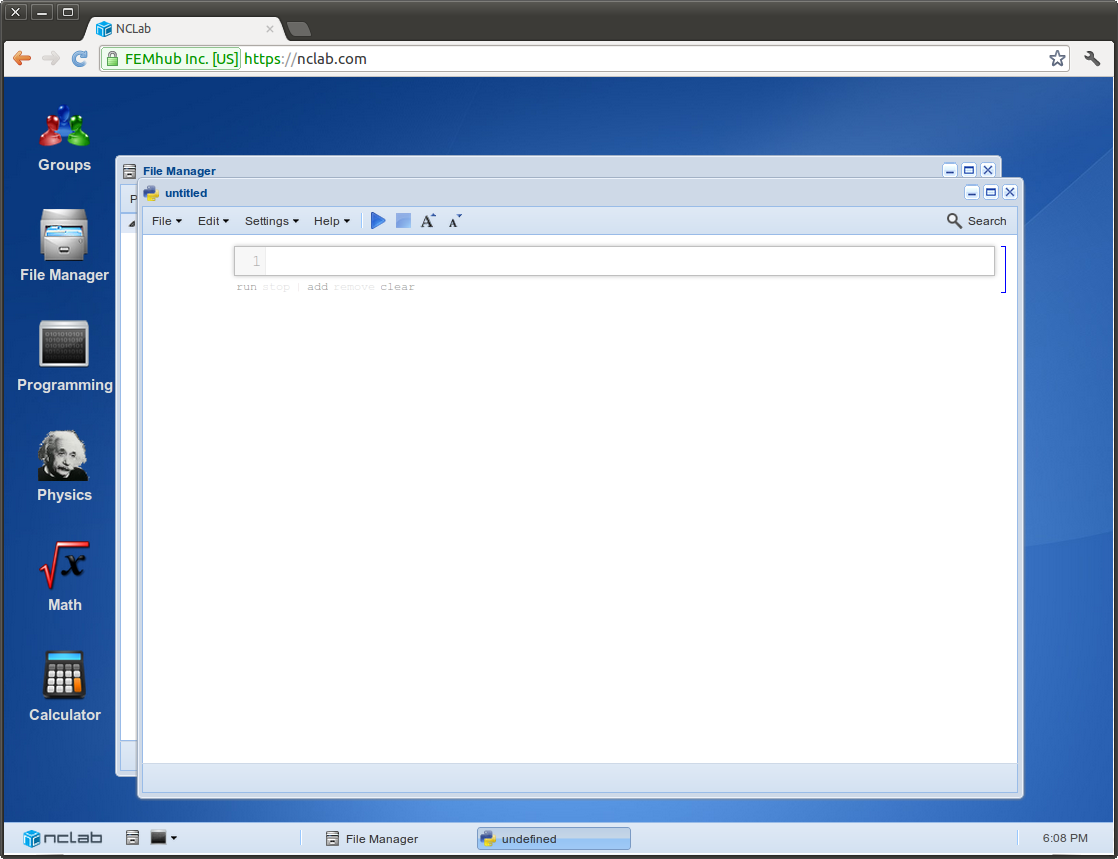
\includegraphics[width=0.9\textwidth]{imgp/python.png}
\end{center}
\vspace{-2mm}
\caption{Launching a new Python project.}
\label{fig:python}
\end{figure}


\subsection{Hello, World!}

Click into the code cell and type {\tt print "Hello, World!"}.
Then click on {\tt run} link under the code cell, and the text 
"Hello, World!" will be displayed 
in a new yellow {\em output cell} as shown in Fig. \ref{fig:python-2}.

\newpage

\begin{figure}[!ht]
\begin{center}
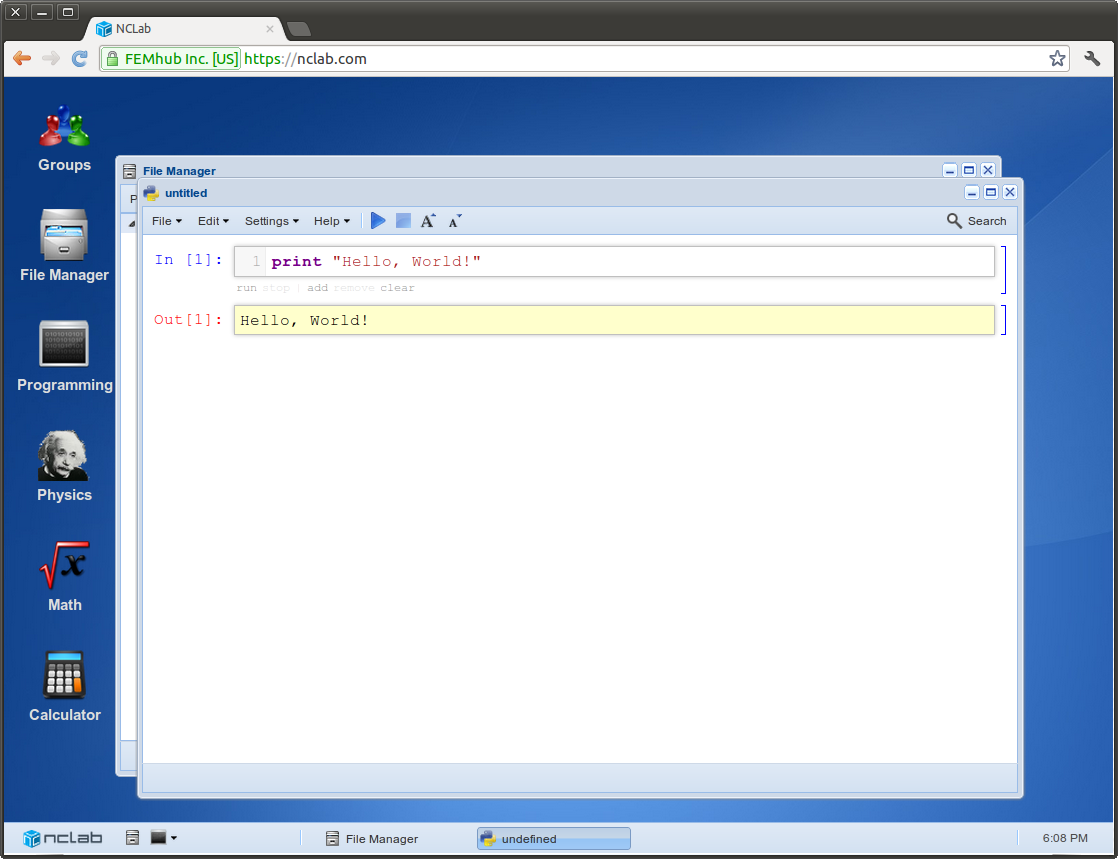
\includegraphics[width=0.9\textwidth]{imgp/python-2.png}
\end{center}
\vspace{-2mm}
\caption{Response received from the cloud is shown in a yellow output cell.}
\label{fig:python-2}
\end{figure}

\subsection{Code, output and text cells}

As in Karel, there are three types of cells in the Python worksheet - code cells, output cells, 
and descriptive text cells. code cells as well as text cells can be added via 
the {\em Edit} menu. New code cells can be also added easily by clicking on {\tt add} under
an existing code cell. code cells and text cells can be removed by clicking on 
{\tt remove} under them. The easiest way to remove a selected output cell is to 
click on it with the mouse and press DELETE on the keyboard. 
All output cells can be removed at once via {\em Remove all output} in the {\em Edit} menu. 

\subsection{Various ways to run programs}

Pressing the green arrow button will run all code cells in the project. Clicking 
on {\tt run} under an code cell will run only the contents of that code cell. 
Same effect can be achieved by holding CTRL and pressing ENTER. Holding SHIFT
and pressing ENTER will evaluate the current code cell and create an additional one
under it.

\section{Using Python as a Graphing Calculator} \label{sec:calc}

\subsection{Objectives}

\begin{itemize}
\item Learn how to use Python for advanced math operations.
\item Plot graphs of functions of one and two variables, as well as parametric 2D and 3D curves.
\end{itemize}
The Python worksheet can be used as a powerful calculator and graphing utility. 
Let us begin with the simplest math operations.

\subsection{Addition, subtraction}

Launch a new Python project and in the code cell type:

\begin{verbatim}
3 + 6
\end{verbatim}
Then click on the {\tt run} link under the code cell. The output should be displayed quickly:

\begin{verbatim}
9
\end{verbatim}
You can add real numbers too,
\begin{verbatim}
3.2 + 6.31
\end{verbatim}
Output:

\begin{verbatim}
9.51
\end{verbatim}
Two numbers can be subtracted as follows,

\begin{verbatim}
7.5 - 2.1
\end{verbatim}
Output:

\begin{verbatim}
5.4
\end{verbatim}

\subsection{Multiplication}
Multiplication is done using the '{\tt *}' symbol as in

\begin{verbatim}
3 * 12
\end{verbatim}
Output:

\begin{verbatim}
36
\end{verbatim}
Of course, real numbers can be multiplied as well:

\begin{verbatim}
3.7 * 12.17
\end{verbatim}
Output:

\begin{verbatim}
45.029
\end{verbatim}
\subsection{Division}
With division, we need to be a bit careful. Look at this:

\begin{verbatim}
30 / 5
\end{verbatim}
Output:

\begin{verbatim}
6
\end{verbatim}
And then look at this:

\begin{verbatim}
33 / 5
\end{verbatim}
Output:

\begin{verbatim}
6
\end{verbatim}
In all major computer languages including C, C++, Fortran, Python and 
others:\\

\begin{center}
\framebox{\color{red}\bf The result of division of two integers is an integer!}
\end{center}

\vspace{4mm}
\noindent
So, when dividing two integers, everything behind the decimal point is lost.
In order to stay on the safe side, 
before you perform division of two numbers, always convert at least one of them
to a real number. This is simple: While {\tt 5} is an integer, {\tt 5.}
and {\tt 5.0} are reals. It is also possible to 
say {\tt float(5)}. In fact this is the best way since it also works for 
variables. Such as, when we are dividing {\tt a / b}, to make sure that 
the result will be correct also for integers, we type {\tt float(a) / b}. 
When at least one number is a real, then the result of the division is a real.   
Variables will be discussed shortly.

\subsection{Powers}
Sometimes we need to use exponents, such as in $2^4$. Python has a double-star
symbol {\tt **} for this:

\begin{verbatim}
2**4
\end{verbatim}
Output:

\begin{verbatim}
16
\end{verbatim}
\subsection{Modulo}
The last of the common arithmetic operations is {\em modulo}. Recall that this is the remainder 
after integer division. In Python modulo is done using the per cent symbol:

\begin{verbatim}
6 % 4
\end{verbatim}
Output:

\begin{verbatim}
2
\end{verbatim}
Of course, one can use brackets:

\begin{verbatim}
5 * (7 - 3)
\end{verbatim}
Output:

\begin{verbatim}
20
\end{verbatim}
\subsection{Order of operations}
Python respects the standard order of operations:

\begin{itemize} 
\item Round brackets have the highest priority,
\item then exponentiation, 
\item then multiplication and division (same priority),
\item the lowest priority have addition and subtraction.
\end{itemize}
Note that no other brackets such as {\tt \{ \}} and {\tt [ ]} are 
admissible in mathematical expressions since they have a different 
function in the programming language.

To illustrate the priority of operations, we can try the following:

\begin{verbatim}
3**4 / 27 * 5 + 3 * 5
\end{verbatim}
Output:

\begin{verbatim}
30
\end{verbatim}
\subsection{Using empty characters makes you code better readable}
Your code will be much better readable if you use empty
characters on either side of arithmetic symbols, as well as 
after commas. Hence, you should never write things like {\tt 3**4/27*5+3*5}.

\subsection{Using mathematical functions}

In order to calculate square roots, exponentials, sines, cosines, tangents, and many other 
math functions, the best way is to import Numpy. Numpy is a powerful Python library 
for numerical computations. To import it, just include the following 
line in your code:

\begin{verbatim}
from numpy import *
\end{verbatim}
Here the symbol '{\tt *}' stands for "everything". If you wanted to import just one or two 
functions, you could do that as well by just giving their names, separated by commas. 

After Numpy is imported, we can calculate, for example, $e^2$:

\begin{verbatim}
exp(2)
\end{verbatim}
Output:
\begin{verbatim}
7.3890560989306504
\end{verbatim}
Elementary functions (and constants) that one can import from Numpy are listed
below. We also show their arguments for clarity, but the functions are imported without 
them. For example, the absolute value function is imported via {\tt from numpy import abs}.\\

%{\small
\begin{center}
\begin{tabular}{|l|l|}
\hline
pi &  $\pi$\\
abs($x$) &  absolute value of $x$\\
arccos($x$) &  inverse cosine of $x$ \\
arccosh($x$) &  inverse hyperbolic cosine of $x$ \\
arcsin($x$) & inverse sine of $x$ \\
arcsinh($x$) & inverse hyperbolic sine of $x$ \\
arctan($x$) & inverse tangent of $x$ \\
arctanh($x$) & inverse hyperbolic tangent of $x$ \\
arctan2($x_1$, $x_2$) & arc tangent of $x_1/x_2$ choosing the quadrant correctly \\
cos($x$) & cosine of $x$ \\
cosh($x$) & hyperbolic tangent of $x$ \\
exp($x$) & $e^x$ \\
log($x$) & natural logarithm of $x$ \\
pow($a$, $b$) & $a^b$ (same as "a**b")\\
sin($x$) & sine of $x$ \\
sinh($x$) & hyperbolic sine of $x$ \\
sqrt($x$) & square root of $x$ \\
tan($x$) & tangent of $x$\\
tanh($x$) & hyperbolic tangent of $x$ \\
\hline
\end{tabular}
\end{center}
%}
\vspace{4mm}
\noindent

\subsection{\ \ Complex numbers}
Complex numbers are always represented as two floating point numbers, the 
real and imaginary part. Appending '{\tt j}' or  '{\tt J}' to a real number
makes it imaginary:

\begin{verbatim}
1j * 1J
\end{verbatim}
Output:

\begin{verbatim}
(-1+0j)
\end{verbatim}
This is one way to define complex numbers:
\begin{verbatim}
1 + 3j
\end{verbatim}
Output:

\begin{verbatim}
(1+3j)
\end{verbatim}
Another way is to use the command {\tt complex}:

\begin{verbatim}
complex(1, 3)
\end{verbatim}
Output:

\begin{verbatim}
(1+3j)
\end{verbatim}
All arithmetic operations that are used for real numbers can be 
used for complex numbers as well, for example:

\begin{verbatim}
(1 + 2j) / (1 + 1j)
\end{verbatim}
Output:

\begin{verbatim}
(1.5+0.5j)
\end{verbatim}
To extract the real and imaginary parts of a complex number {\tt z}, use {\tt z.real}
and {\tt z.imag}. Use {\tt abs()} to get the absolute value:

\begin{verbatim}
a = 3 + 4j
a.real
a.imag
abs(a)
\end{verbatim}
Output:

\begin{verbatim}
3
4
5
\end{verbatim}


\subsection{\ \ Plotting functions of one variable}\label{plotting}

Plotting can be done via the Pylab library. The Pylab {\tt plot} command takes two
arrays: $x$-coordinates and $y$-coordinates of points on a curve. Between the 
points, the curve is interpolated linearly. Let us illustrate this on a simple 
example with just five points [0, 0], [1, 2], [2, 0.5], [3, 2.5] and [4, 0]:

\begin{verbatim}
from pylab import *
x = [0,0, 1.0, 2.0, 3.0, 4.0]
y = [0.0, 2.0, 0.5, 2.5, 0]
clf()
plot(x, y)
lab.show()
\end{verbatim}
The commands {\tt clf()}, {\tt plot()} and {\tt lab.show()} do clear the canvas, 
plot the graph, and show the graph, respectively.
The output is shown in Fig. \ref{fig:plot}.


\begin{figure}[!ht]
\begin{center}
\hbox{}
\hspace{-6mm}
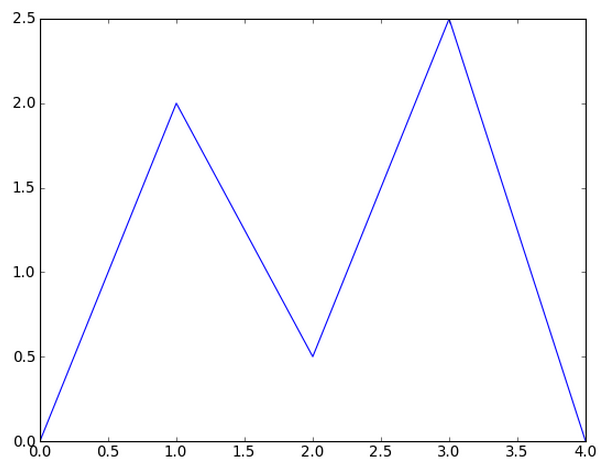
\includegraphics[width=0.56\textwidth]{imgp/plot.png}
\end{center}
\vspace{-2mm}
\caption{Piecewise-linear curve with five points.}
\label{fig:plot}
%\vspace{-1cm}
\end{figure}
\noindent
In the following we will discuss more options and show some useful techniques.
Let's say, for example, that we want to plot the function $f(x) = \sin(x)$
in the interval $(0, 2\pi)$. The array of $x$-coordinates of equidistant points 
between 0 and $\pi$ with step 0.05 can be created easily using the command {\tt arange}:

\begin{verbatim}
from numpy import *
x = arange(0, 2*pi, 0.05)
\end{verbatim}
Changing the step size will change the resolution - with a smaller step the resolution will 
be finer and vice-versa. Next, the array of $y$-coordinates of the points is obtained via

\begin{verbatim}
y = sin(x)
\end{verbatim}
The last part we already know:

\begin{verbatim}
clf()
plot(x, y)
lab.show()
\end{verbatim}
\noindent
The output is shown in Fig. \ref{fig:plot1}.\\[-7mm]

\begin{figure}[!ht]
\begin{center}
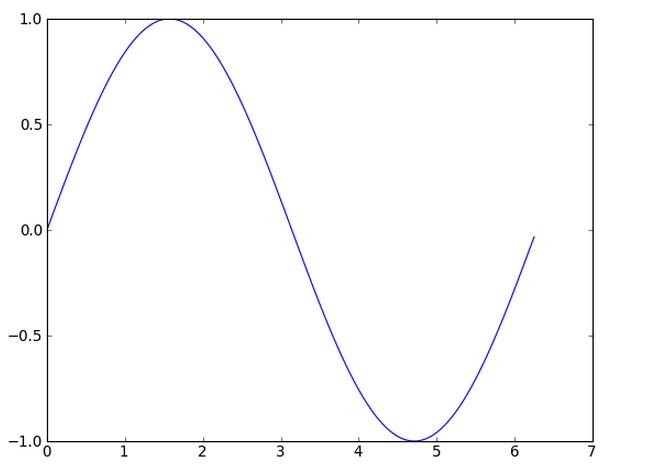
\includegraphics[width=0.6\textwidth]{imgp/plot1.png}
\end{center}
\vspace{-6mm}
\caption{Plotting $\sin(x)$ in interval $(0, 2\pi)$ with subdivision step 0.05.}
\label{fig:plot1}
\vspace{-2mm}
\end{figure}
\noindent

\subsection{\ \ Labels, colors, and styles}

The plot can be made nicer by adding a label, and also the color 
and the line style can be changed. Let us start with adding a label:

\begin{verbatim}
plot(x, y, 'b-', label = "Solid blue line")
legend()
lab.show()
\end{verbatim}
The output is shown in Fig. \ref{fig:plot2}.\\[-7mm]

\begin{figure}[!ht]
\begin{center}
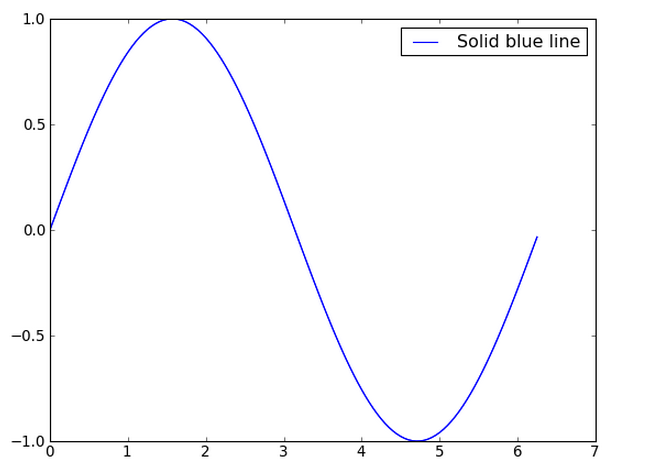
\includegraphics[width=0.6\textwidth]{imgp/plot2.png}
\end{center}
\vspace{-6mm}
\caption{Adding a label.}
\label{fig:plot2}
%\vspace{-1cm}
\end{figure}
\newpage
\noindent
Next let us change the color to red and line style to dashed: 

\begin{verbatim}
clf()
plot(x, y, 'r--', label = "Dashed red line")
legend()
lab.show()
\end{verbatim}
The output is shown in Fig. \ref{fig:plot3}.\\[-7mm]


\begin{figure}[!ht]
\begin{center}
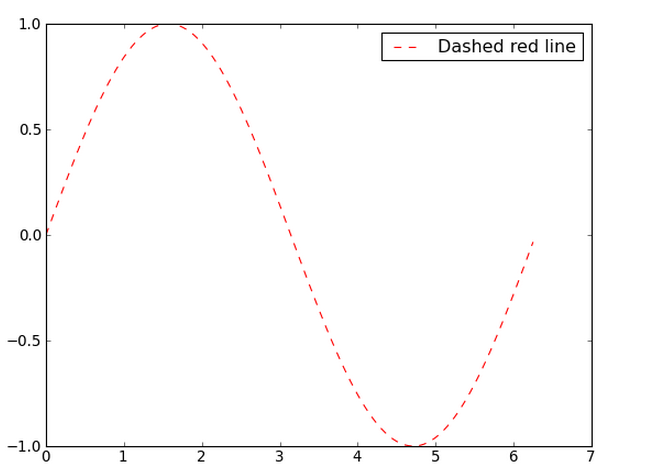
\includegraphics[width=0.6\textwidth]{imgp/plot3.png}
\end{center}
\vspace{-6mm}
\caption{Same graph using dashed red line.}
\vspace{-1cm}
\label{fig:plot3}
\end{figure}
\newpage
\noindent
The graph can be plotted using green color and small dots rather than 
a solid or dashed line:

\begin{verbatim}
clf()
plot(x, y, 'g.', label = "Dotted green line")
legend()
lab.show()
\end{verbatim}
The output is shown in Fig. \ref{fig:plot4}.

\begin{figure}[!ht]
\begin{center}
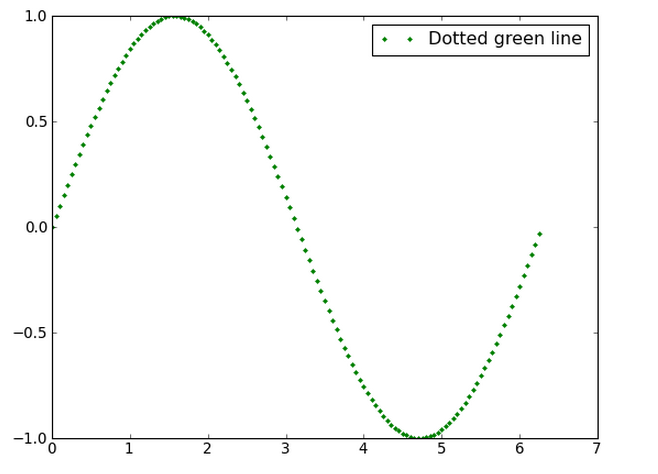
\includegraphics[width=0.6\textwidth]{imgp/plot4.png}
\end{center}
\vspace{-6mm}
\caption{Same graph using dotted green line.}
\label{fig:plot4}
%\vspace{-5mm}
\end{figure}
\noindent
\noindent
Last let us stay with green color but make the dots larger:

\begin{verbatim}
clf()
plot(x, y, 'go', label = "Bigger green dots")
legend()
lab.show()
\end{verbatim}
\noindent
The output is shown in Fig. \ref{fig:plot5}.
\newpage

\begin{figure}[!ht]
\begin{center}
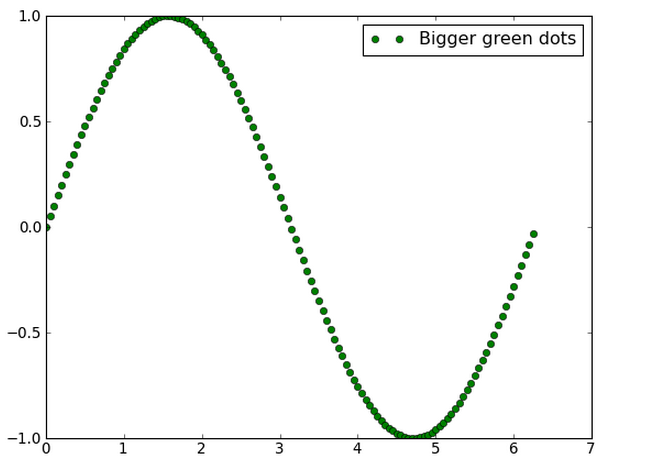
\includegraphics[width=0.6\textwidth]{imgp/plot5.png}
\end{center}
\vspace{-6mm}
\caption{Same graph using large green dots.}
\label{fig:plot5}
%\vspace{-4mm}
\end{figure}
\noindent

\subsection{\ \ Scaling axes and showing grid}

In the previous plots, function graphs were fitted into the 
display window, which means that the horizontal and vertical 
axes were scaled differently. This can be changed by including the 
{\tt axis('equal')} command after calling {\tt plot()}. Also, 
grid can be displayed by using the {\tt grid()} command:

\begin{verbatim}
from numpy import *
from pylab import *
x = arange(0, 2*pi, 0.05)
y = sin(x)
clf()
plot(x, y, label="sin(x)")
axis('equal')
grid()
legend()
lab.show()
\end{verbatim}
\noindent
The output is shown in Fig. \ref{fig:plot8}.
\newpage

\begin{figure}[!ht]
\begin{center}
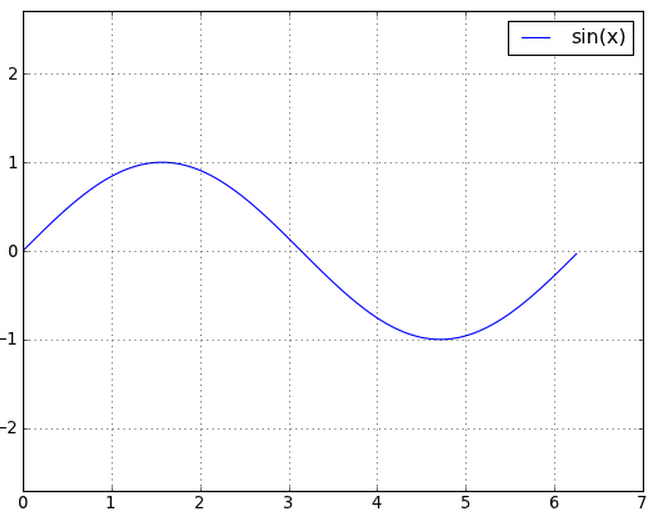
\includegraphics[width=0.53\textwidth]{imgp/plot8.png}
\end{center}
\vspace{-4mm}
\caption{Scaling axes equally and showing grid.}
\label{fig:plot8}
\vspace{-2mm}
\end{figure}
\noindent
The scaling of axes can be returned to the automatic fit option via
{\tt axis('auto')} if needed.

\subsection{\ \ Adjusting plot limits}

Plot limits can be set using the {\tt xlim()} and {\tt ylim()}
functions after {\tt plot()}. For example, we can stretch the sine
function from Fig. \ref{fig:plot8} to span the entire width of the 
canvas as follows:

\begin{verbatim}
from numpy import *
from pylab import *
x = arange(0, 2*pi, 0.05)
y = sin(x)
clf()
plot(x, y, label="sin(x)")
xlim(0, 2*pi)
axis('equal')
grid()
legend()
lab.show()
\end{verbatim}
\noindent
The output is shown in Fig. \ref{fig:plot9}.
\newpage

\begin{figure}[!ht]
\begin{center}
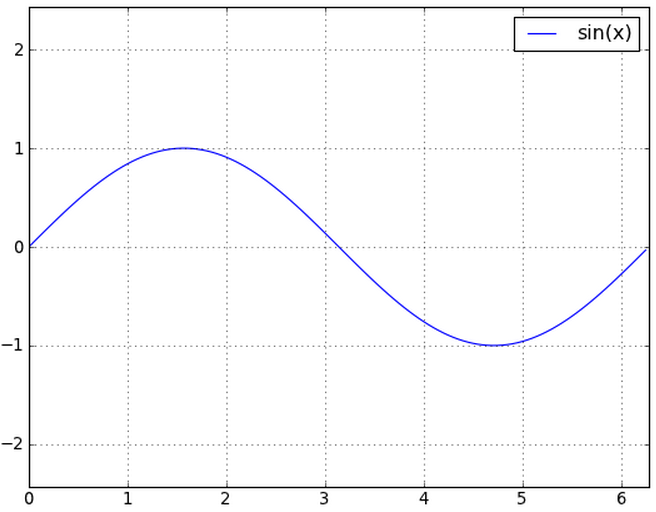
\includegraphics[width=0.53\textwidth]{imgp/plot9.png}
\end{center}
\vspace{-4mm}
\caption{Setting plot linits on the horizontal axis to $0$ and $2\pi$.}
\label{fig:plot9}
\vspace{-2mm}
\end{figure}
\noindent


\subsection{\ \ Plotting multiple functions at once}

This can be done very easily, just do not use the {\tt clf()}
command between the plots and you can have as many graphs 
in one figure as needed. Let us do three:

\begin{verbatim}
from numpy import *
from pylab import *
x = arange(0.5, 5, 0.05)
y1 = 1./x
y2 = 1. / (1 + x**2)
y3 = exp(-x)
axis=("equal")
clf()
plot(x, y1, label="y1")
plot(x, y2, label="y2")
plot(x, y3, label="y3")
legend()
lab.show()
\end{verbatim}
\noindent
The output is shown in Fig. \ref{fig:plot7}.
\newpage

\begin{figure}[!ht]
\begin{center}
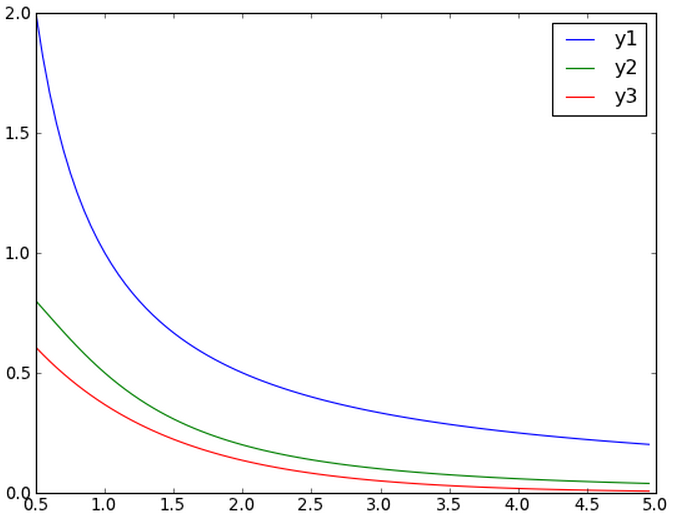
\includegraphics[width=0.54\textwidth]{imgp/plot7.png}
\end{center}
\vspace{-4mm}
\caption{Plotting graphs of functions $1/x$, $1 / (1 + x^2)$ and $e^{-x}$ in interval $(0.5, 5)$.}
\label{fig:plot7}
\vspace{-2mm}
\end{figure}
\noindent
The {\tt plot()} command in Pylab is much more powerful, we just saw a small 
fraction of its functionality. For a complete list of options 
visit the Pylab page {\tt http:// www.scipy.org/PyLab}.

\subsection{\ \ Plotting parametric 2D curves}\label{subsec:planarcurves}

The concept of plotting based on two arrays of $x$ and $y$ coordinates
allows us to do much more than only plot graphs of functions of one variable.
We can easily plot more general curves such as circles, spirals and others.
Let us illustrate this on a spiral that is parameterized 
by 
$$
x(t) = t \cos(t), \ \ \ \ 
y(t) = t \sin(t)
$$ 
in the interval $(0, 10)$ for $t$. The complete code is

\begin{verbatim}
from pylab import *
from numpy import *
t = arange(0, 10, 0.05)
x = t*cos(t)
y = t*sin(t)
clf()
plot(x, y)
lab.show()
\end{verbatim}
The output is shown in Fig. \ref{fig:plot6}.

\begin{figure}[!ht]
\begin{center}
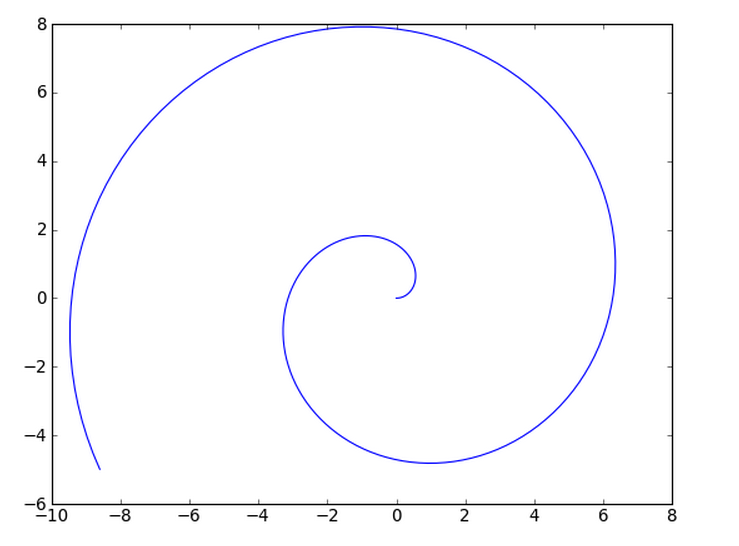
\includegraphics[width=0.6\textwidth]{imgp/plot6.png}
\end{center}
\vspace{-6mm}
\caption{Plotting a spiral.}
\label{fig:plot6}
\vspace{-0mm}
\end{figure}
\noindent

\subsection{\ \ Plotting parametric 3D curves}

For 3D plots it is practical to use the {\tt mplot3d} toolkit of the 
Python library Matplotlib. Let us begin with 
parametric 3D curves since this is analogous to how we handled planar curves in 
the previous paragraph. 3D curves are sequences of linearly interpolated 3D points
represented via three arrays of $x$, $y$ and $z$ coordinates. As an 
example we will plot the curve $x(t), y(t), z(t)$ where

$$
x(t) = (1 + t^2) \sin(2 \pi t), \ \ \ y(t) = (1 + t^2) \cos(2 \pi t), \ \ \ z(t) = t,
$$
and where the parameter $t$ lies in the interval $(-2, 2)$.

\begin{verbatim}
# Import Numpy and Matplotlib:
from numpy import *
import matplotlib as mpl
from mpl_toolkits.mplot3d import Axes3D
import matplotlib.pyplot as plt

# Set legend font size (optional):
mpl.rcParams['legend.fontsize'] = 15

# Setup the 3D plot:
fig = plt.figure()
ax = fig.gca(projection='3d')

# Define interval for parameter 't' and its
# division (arange can be used as well):
t = linspace(-2, 2, 100)

# Define the curve:
x = (1 + t**2) * sin(2 * pi * t)
y = (1 + t**2) * cos(2 * pi * t)
z = t

# Plot the curve
ax.plot(x, y, z, label='Parametric 3D curve')
ax.legend()

# Show the plot:
lab.show()
\end{verbatim}
The output is shown in Fig. \ref{fig:plot3d-1}.

\begin{figure}[!ht]
\begin{center}
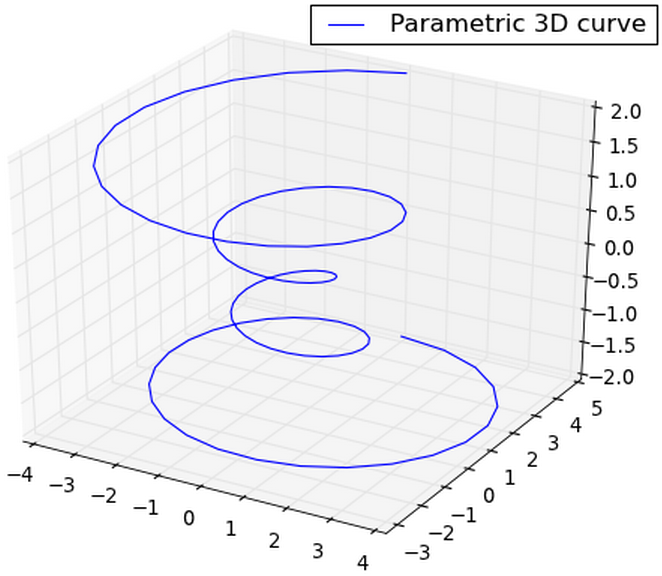
\includegraphics[width=0.6\textwidth]{imgp/plot3d-1.png}
\end{center}
\vspace{-4mm}
\caption{Plotting a parametric 3D curve.}
\label{fig:plot3d-1}
%\vspace{-1cm}
\end{figure}


\subsection{\ \ Plotting functions of two variables}

There are several ways to plot graphs of functions of two variables, 
first let us do this with Matplotlib's {\tt mplot3d} toolkit, then we will
use WebGL. We will plot the graph of the function 

$$
  f(x, y) = \sin(x) \sin(y)
$$
in the square $(-\pi, \pi) \times (-\pi, \pi)$.

\begin{verbatim}
# Import Numpy and Matplotlib:
from numpy import *
from mpl_toolkits.mplot3d import axes3d
import matplotlib.pyplot as plt

# Setup the 3D plot:
fig = plt.figure()
ax = fig.gca(projection='3d')

# Define intervals on the 'x' and 'y' axes and 
# their divisions (arange can be used as well):
x = linspace(-pi, pi, 30)
y = linspace(-pi, pi, 30)

# Create Cartesian grid:
X, Y = meshgrid(x, y)

# Calculate values at grid points:
Z = sin(X) * sin(Y)

# Plot the data:
ax.plot_wireframe(X, Y, Z, rstride=1, cstride=1)

# Show the plot:
lab.show()
\end{verbatim}
The parameters {\tt rstride} (row stride) and {\tt cstride} (column stride)
can be used to make the plot coarser when they are set to 2, 3, etc.
The output is shown in Fig. \ref{fig:plot3d-2}.
\newpage

\begin{figure}[!ht]
\begin{center}
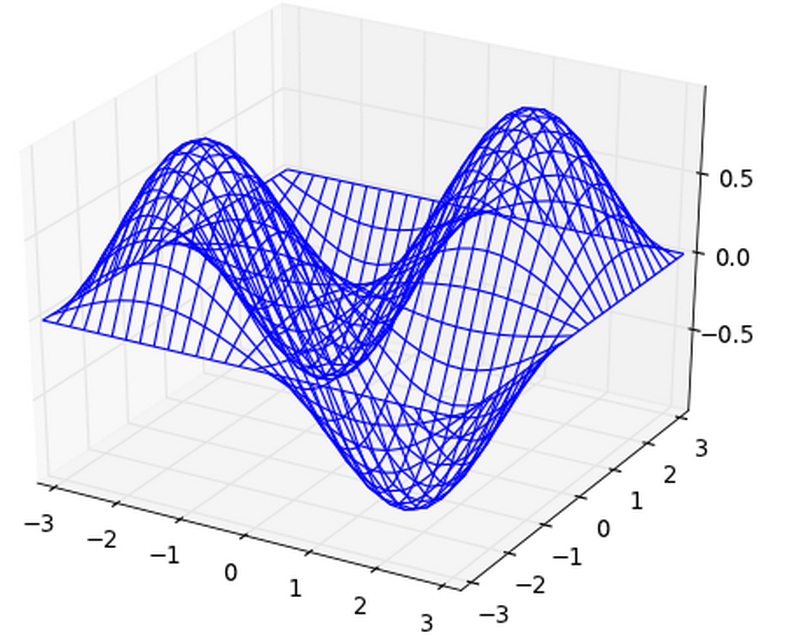
\includegraphics[width=0.6\textwidth]{imgp/plot3d-2.png}
\end{center}
\vspace{-4mm}
\caption{Wireframe plot of the function $f(x, y)$.}
\label{fig:plot3d-2}
%\vspace{-1cm}
\end{figure}
\noindent
Solid surface plot can be obtained by replacing in the above code 
{\tt plot\_wireframe} with {\tt plot\_surface}. 
The output is shown in Fig. \ref{fig:plot3d-3}.

\begin{figure}[!ht]
\begin{center}
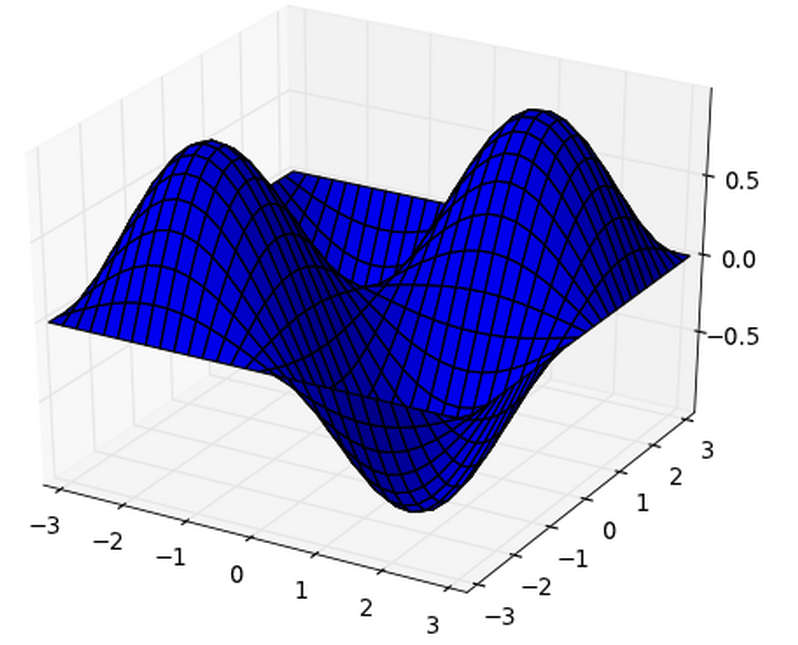
\includegraphics[width=0.6\textwidth]{imgp/plot3d-3.png}
\end{center}
\vspace{-4mm}
\caption{Surface plot of the function $f(x, y)$.}
\label{fig:plot3d-3}
%\vspace{-1cm}
\end{figure}
\newpage

\noindent
Contour plot can be obtained by replacing in the above code 
the line 

\begin{verbatim}
ax.plot_wireframe(X, Y, Z, rstride=1, cstride=1)
\end{verbatim}
with 

\begin{verbatim}
cset = ax.contour(X, Y, Z)
ax.clabel(cset)
\end{verbatim}
The output is shown in Fig. \ref{fig:plot3d-4}.

\begin{figure}[!ht]
\begin{center}
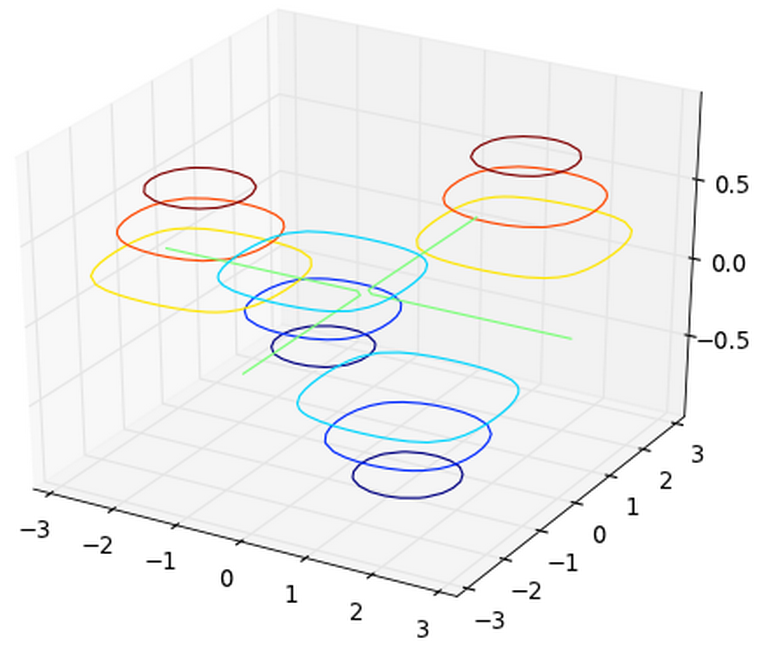
\includegraphics[width=0.6\textwidth]{imgp/plot3d-4.png}
\end{center}
\vspace{-4mm}
\caption{Contour plot of the function $f(x, y)$.}
\label{fig:plot3d-4}
%\vspace{-1cm}
\end{figure}
\noindent
We have only mentioned the most basic Matplotlib's functionality, for more options 
we refer to the tutorial 
at {\tt http://matplotlib.sourceforge.net/mpl\_toolkits/mplot3d}.


\subsection{\ \ Plotting functions of two variables with WebGL}

For this functionality, your browser has to support WebGL (most of modern browsers do, 
with the exception of Internet Explorer). See the introductory tutorial {\em Welcome to NCLab}
on the page {\tt http://femhub.com/nclab-tutorials/} for detailed instructions on how to enable WebGL. 
In the following example, we plot the graph of the function 

$$
  f(x, y) = \sin(\sqrt{x^2 + y^2})
$$
in the square $(0, 10) \times (0, 10)$.

\begin{verbatim}
from numpy import sin, sqrt, arctan

# Define intervals on the x and y axes.
x0 = 0.0
x1 = 10.0
y0 = 0.0
y1 = 10.0

# Define the corresponding divisions.
nx = 100
ny = 100

# Define the function:
def f(x, y):
    return sin(sqrt(x**2 + y**2))

# Render the surface using WebGL.
lab.surface((x0, x1, nx), (y0, y1, ny), f)
\end{verbatim}
The output is shown in Fig. \ref{fig:webgl}.

\begin{figure}[!ht]
\begin{center}
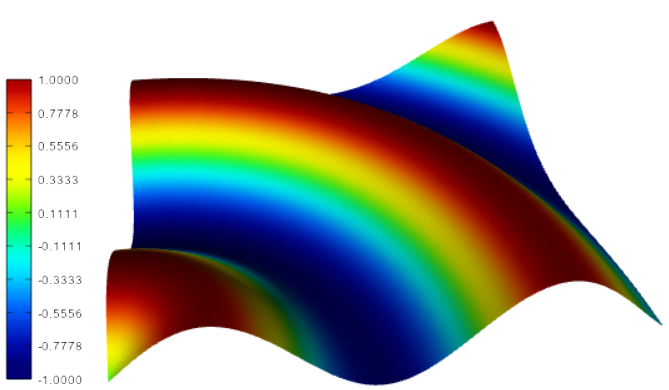
\includegraphics[width=0.6\textwidth]{imgp/webgl.png}
\end{center}
\vspace{-2mm}
\caption{Plotting functions of two variables with WebGL.}
\label{fig:webgl}
%\vspace{-1cm}
\end{figure}

%%%%%%%%%%%%%%%%%%%%%%%%%%%%%%%%%%%%%%%%%%%%%%%%%%%%%%%%%%%%%%%%%%%%%%%%%%%

\section{More on Functions}

\subsection{Objectives}

\begin{itemize}
\item Review and refine your knowledge of functions.
\item Learn to use default arguments and return multiple values.
\end{itemize}
Custom {\em functions} in Python are the same thing as in Karel, 
but in Python they can moreover {\em accept arguments}. Recall that 
functions in Karel were defined to make some functionality easily 
reusable -- in Python they are defined for the same reason.

\subsection{Defining new functions}

Definition of a new function begins with the keyword {\tt def} as in Karel. In Python,
we moreover use round brackets for arguments and a colon at the end of the line. 
For example, the following function adds two numbers
and returns the result:

\begin{verbatim}
def add(a, b):
    return a + b
\end{verbatim}
The round brackets in the function definition are mandatory even if no arguments are passed,
and the {\tt return} statement can be omitted if not needed.
The two lines of code above 
are a {\em function declaration} -- they do not produce any output.
In order to call the function, we need to write one additional line, such as:

\begin{verbatim}
print "5 + 3 is", add(5, 3)
\end{verbatim}
This will produce the following output:

\begin{verbatim}
5 + 3 is 8
\end{verbatim}
To show another example, the following function does not take any arguments 
and it does not return any results:

\begin{verbatim}
def hello():
    print "Hello!"
\end{verbatim}

\subsection{Passing arbitrary arguments}

Python does not require that we specify the type of function arguments. 
What does it mean? The above function {\tt add(a, b)} works for real
numbers, complex numbers, vectors, strings, and any other 
objects where the operation '+' is defined. Let's try this:

\begin{verbatim}
def add(a, b):
    return a + b

word1 = "Good "
word2 = "Evening!"
print add(word1, word2)
\end{verbatim}
Output:

\begin{verbatim}
Good Evening!
\end{verbatim}
Things like this make Python very intuitive and easy to use. In conventional languages such as C or C++, 
we would have to define different functions: {\tt add\_real\_numbers(a, b)} for real numbers,
{\tt add\_complex\_numbers(a, b)} for complex numbers numbers, {\tt add\_strings(a, b)} for strings, etc. 
In C, they would be as follows:

\begin{verbatim}
double add_real_numbers(double a, double b)
{
  return a + b;
}
\end{verbatim}
and

\begin{verbatim}
# include <complex.h>
complex add_complex_numbers(complex a, complex b)
{
  return a + b;
}
\end{verbatim}
and 

\begin{verbatim}
void add_strings(const char* a_in, const char* b_in, char* c_out)
{
  strcpy(c_out, a_in);
  strcat(c_out, b_in);
  return;
}
\end{verbatim}

\subsection{Returning multiple values}

Python functions can return multiple values which often comes handy.
For example, the following function returns the 
second, third, and fourth powers of a number:

\begin{verbatim}
def powers(a):
    return a**2, a**3, a**4
\end{verbatim}
This is how the function is used:

\begin{verbatim}
var1 = 2
print "Powers are", powers(var1)
\end{verbatim}
Output:

\begin{verbatim}
Powers are (4, 8, 16)
\end{verbatim}
We can also store the returned values in three separate variables:

\begin{verbatim}
var1 = 3
p2, p3, p4 = powers(var1)
print "Powers are", p2, p3, p4
\end{verbatim}
Output:

\begin{verbatim}
Powers are 9 27 81
\end{verbatim}
Look how complicated the same program would be in C/C++:

\begin{verbatim}
void powers(double a, double* p2, double* p2, double* p3)
{
  *p2 = pow(a, 2);
  *p3 = pow(a, 3);
  *p4 = pow(a, 4);
  return;
}

int main()
{
  double p1, p2, p3;
  double a = 2;
  powers(a, &p2, &p2, &p3);
  printf("Powers are %g, %g, %g.\n", p2, p3, p4);
}
\end{verbatim}

\subsection{Using default arguments}

Holland is the most bicycle friendly country in the world. Imagine that you 
work for the Holland Census Bureau. Your task is to ask 10000 
people how they go to work, and enter their answers into a database. 
The program for entering data into the database was written by one of 
your colleagues, and it can be used as follows:

\begin{verbatim}
add_database_entry("John", "Smith", "walks")
\end{verbatim}
or 
\begin{verbatim}
add_database_entry("Louis", "Armstrong", "bicycle")
\end{verbatim}
or
\begin{verbatim}
add_database_entry("Jim", "Bridger", "horse")
\end{verbatim}
etc. Since you are in Holland, it can be expected that $99 \%$ of people 
are using the bicycle. In principle you could call the function {\tt add\_database\_entry()} 
to enter each answer, but with 9900 bicyclists out of 10000 respondents you would have to 
type {\tt "bicycle"} MANY times. 

Fortunately, Python offers a smarter way to do this. We can define a new function 

\begin{verbatim}
def enter(first, last, transport = "bicycle"):
    enter_into_database(first, last, transport)
\end{verbatim}
This is a simple ({\em "thin"}) {\em wrapper} to the function {\tt add\_database\_entry()} 
that allows us to omit the third argument in the function call and autocomplete 
it with a {\em default argument} {\tt "bicycle"}. In other words, now we do not have to 
type {\tt "bicycle"} for Louis Armstrong or any other bicyclist:

\begin{verbatim}
enter("Louis", "Armstrong")
\end{verbatim}
Only if we meet a rare someone who uses a car, we type 

\begin{verbatim}
enter("Niki", "Lauda", "car")
\end{verbatim}
Another example: Let us return to the function {\tt add()}, and let us 
imagine that very often (but not always) the second number that we
are adding is 10. Then it makes sense to write the function {\tt add()}
as follows:

\begin{verbatim}
def add(a, b = 10):
    return a + b
\end{verbatim}
The function will work as before when called with two arguments: 

\begin{verbatim}
A = 5
B = 1
add(A, B)
\end{verbatim}
Output:
\begin{verbatim}
6
\end{verbatim}
But it can be also called with the second argument omitted:
\begin{verbatim}
A = 5
add(A)
\end{verbatim}
Output:
\begin{verbatim}
15
\end{verbatim}
\underline{Some rules to remember}:
\begin{itemize}
\item Default arguments need to be introduced {\bf after} standard (non-default) arguments. In other words, the 
      following code will result into an error:
\begin{verbatim}
def add(a = 5, b):
    return a + b
\end{verbatim}
This is the error message:
\begin{verbatim}
  File "<nclab>", line 1
SyntaxError: non-default argument follows default argument

\end{verbatim}
\item If multiple default arguments are present, they have to follow the non-default ones.
      If the number of arguments in the function call is less than the total number of default and non-default
      arguments, then first all non-default arguments are assigned, and then the default ones from 
      left to right. To illustrate this, assume the function:
\begin{verbatim}
def add(x, a = 2, b = 3):
    return x + a + b
\end{verbatim}
This function can be called as follows:
\begin{verbatim}
print add(1)
\end{verbatim}
In this case, the value {\tt 1} is assigned to {\tt x} and {\tt a} and {\tt b} take the default values.
The output will be 
\begin{verbatim}
6
\end{verbatim}
When the function is called with just two values,
\begin{verbatim}
print add(5, 6)
\end{verbatim}
then the value {\tt 5} is assigned to {\tt x}, {\tt 6} to {\tt a}, and {\tt b} takes the default value {\tt 3}.
The output is
\begin{verbatim}
14
\end{verbatim}
However, it is always a good idea to be as transparent as possible. Therefore a better code is 
\begin{verbatim}
print add(1, a = 6)
\end{verbatim}
Then the result is the same, {\tt 14}, but it is clear even to non-experts what is going on. Moreover,
in this way we can also define the value of {\tt b} without having to define the value of {\tt a}:
\begin{verbatim}
print add(1, b = 6)
\end{verbatim}
Now {\tt x} is {\tt 1}, {\tt a} has the default value {\tt 2} and the result is {\tt 9}.
\end{itemize}

\subsection{Programming exercises}

\begin{enumerate}
\item Write a Python function {\tt circle} that accept an arbitrary positive radius $R > 0$
      as argument, and returns the area and the perimeter of a circle with radius $R$.
\item Write a Python function {\tt squarearea} that returns the area of a square whose 
      edge is $a$ cm long. You know that most of the time the edge length wil be 1 cm,
      so make this function callable without any arguments.
\item Write a Python function {\tt rectanglearea} that returns the area of a rectangle 
      whose edges are $a$ and $b$ cm long. You know that most of the time one of the edges 
      will measure 3 cm, so make the function callable with only one argument.
\end{enumerate}

\section{More on Variables}

\subsection{Objectives}

\begin{itemize}
\item Review and refine your knowledge of variables.
\item Understand dynamic type interpretation.
\item Learn about {\em local} and {\em global} variables.
\item Understand why global variables should be avoided.
\item Learn about {\em shadowing} of variables.
\end{itemize}
The reason why we use variables is the same in Karel the Robot, Python, and all other programming 
languages -- to store useful information for later use. Also the way we work with variables is almost the 
same, so we will just mention a few aspects that are new in Python.

\subsection{Assigning values to variables}

In Python, several variables can be initialized at the same time:

\begin{verbatim}
x = y = z = 0.0
print "x =", x
print "y =", y
print "z =", z
\end{verbatim}
Output:

\begin{verbatim}
x = 0.0
y = 0.0
z = 0.0
\end{verbatim}
As in Karel, variables must be defined (have a value assigned) before they can be 
used. 

\subsection{Dynamic type interpretation}

Python is very generous with the types of variables -- it will figure out the type of a variable 
at runtime, depending on the value that we store in it. The type can even change at runtime.
For example, let us look at the following code:

\begin{verbatim}
a = 5
print a
a = "Hi!"
print a
a = True
print a
\end{verbatim}
The output is 

\begin{verbatim}
5
Hi!
True
\end{verbatim}
This is very different from compiled languages such as C, C++ where one needs to declare the type 
of every variable before its first use, and the type then cannot be changed. 

\subsection{Changing values of variables}

The simplest way to increase the value of a numerical variable in Python by a given number 
is to use the '{\tt +=}' command:

\begin{verbatim}
v = 1
v += 3
print "v =", v
\end{verbatim}
Output:

\begin{verbatim}
v = 4
\end{verbatim}
We can also subtract a number from a numerical variable:

\begin{verbatim}
v -= 1
print "New value of v is", v
\end{verbatim}
Output:

\begin{verbatim}
New value of v is 3
\end{verbatim}
We can multiply a numerical variable with a number:

\begin{verbatim}
v *= 4
print "Now v is", v
\end{verbatim}
Output:

\begin{verbatim}
Now v is 12
\end{verbatim}
And finally, we can divide a numerical variable with a number:

\begin{verbatim}
v /= 6
print "Finally, v is", v
\end{verbatim}
Output:

\begin{verbatim}
Finally, v is 2
\end{verbatim}
It is possible to use existing variables to assign a value to a new variable:

\begin{verbatim}
a = 1
b = 2.5
c = 0.5
d = (a + b) / c
print "d =", d
\end{verbatim}
Output:

\begin{verbatim}
d = 7.0
\end{verbatim}
Of course, apples cannot be mixed with oranges. When we try to 
add a number to a text string,

\begin{verbatim}
a = "My car is a Ferrari."
b = 3.5

c = a + b
\end{verbatim}
then the interpreter rightfully complains:

\begin{verbatim}
Traceback (most recent call last):
  File "<nclab>", line 4, in <module>
TypeError: cannot concatenate 'str' and 'float' objects
\end{verbatim}

\subsection{Local and global variables}

If a variable was defined inside of a function, then it is {\em local} to that
function. Imagine a lake -- a fish born in a lake will always 
stay in that lake (fishing neglected). If we try to access 
the variable outside that function, even though the function was 
already called, the variable will be unknown. Look at the following 
code:

\begin{verbatim}
def add(a, b):
    c = a + b
    return c

print "Sum of 3 and 4 is", add(3, 4)
print c
\end{verbatim}
The output is:

\begin{verbatim}
Sum of 3 and 4 is 7
Traceback (most recent call last):
  File "<nclab>", line 6, in <module>
NameError: name 'c' is not defined
\end{verbatim}
In computer programming, {\em we want all our variables to be local}, because 
this avoids name clashes and minimizes the risk of unwanted side effects.
Mistakes such as unwanted overwriting of the value stored in a global variable 
belong to the most difficult ones to find.

\subsection{Sure method to spoil your code}

Once a variable is used in the main program, 
then it is {\em global}, meaning that you could use it in 
any function that you define. Like in the following 
code:

\begin{verbatim}
val = 5.0

def msg():
    print "val =", val

msg()
\end{verbatim}
Brrr, this code is ugly! But it works (unfortunately), see the output:

\begin{verbatim}
val = 5.0
\end{verbatim}
Remember:\\

\begin{center}
{\em Passing global variables to functions is a bad habit that makes your code\\
     difficult to understand, prone to mistakes, and extremely difficult to fix}.\\
\end{center}
\vspace{4mm}
\noindent
A function should always
obtain all the data it needs through its arguments. Imagine that a unit of soldiers 
would act based not only on orders it receives (that's the argument 
list), but also based on rumors that some of the soldiers read in a Sunday magazine. 
That might not work well!\\

\noindent
A clean version of the above code is

\begin{verbatim}
def msg(v):
    print "val =", v

val = 5.0

msg(val)
\end{verbatim}
Can you see the difference? Now the function {\tt msg} is {\em readable} -- you do not 
need to look elsewhere in the program to understand what it does. The output is:

\begin{verbatim}
val = 5.0
\end{verbatim}

\subsection{Variable shadowing}

Sometimes, by accident or intentionally, we may have two different 
variables of the same name in the code. Look, for example, at this short program:

\begin{verbatim}
c = 5

def add(a, b):
    c = a + b
    print "c =", c
    return c

add(1, 2)
print "c =", c
\end{verbatim}
The output is

\begin{verbatim}
c = 3
c = 5
\end{verbatim}
There is no 
problem with the last line of the program because the local variable {\tt c}, defined
inside of the function {\tt add}, is no longer defined there. But inside of the function
{\tt add}, both the global variable {\tt c} and the local variable {\tt c} are defined at 
the same time. This is commonly referred to as {\em variable shadowing}, and we need to 
remember that if this happens, {\bf the local variable is used}.



\subsection{Programming exercises}

\begin{enumerate}
\item The number $\pi$ can be written as an infinite series 
$$
\pi = 4\left(1 - \frac{1}{3} + \frac{1}{5} - \frac{1}{7} + \frac{1}{9} - \ldots     \right).
$$
Write a Python function {\tt approx\_pi()} that returns an approximation of $\pi$ using a truncated 
series where the last fraction used is $1/13$.
\item {\em Arithmetic sequence} is a progression of $n$ numbers $a_1$, $a_2$, $\ldots$, $a_n$
that increase by the same difference $d$. For example, 
$$
5, 7, 9, 11, 13, 15, 17
$$
is an arithmetic sequence with $n = 7$, $a_1 = 5$ and $d = 2$. It holds
$$
a_n = a_1 + (n-1)d.
$$
There is a well known formula for the sum of such a sequence:
$$
S = \frac{n}{2}(a_1 + a_n).
$$
And now the exercise: Write a function {\tt summation\_arithmetic(n, a1, d)} that takes arbitrary 
values of $n$, $a_1$ and $d$ as arguments, and calculates and returns the sum
of the corresponding arithmetic sequence! 
\item {\em Geometric sequence} is a progression of $n$ numbers $a_1$, $a_2$, $\ldots$, $a_n$
where the next number is calculated by multiplying the last one with a quotient $q$.
For example, 
$$
1, \frac{1}{2}, \frac{1}{4}, \frac{1}{8}, \frac{1}{16}
$$
is a geometric sequence with $n = 5$, $a_1 = 1$ and $q = 1/2$. It is 
$$
a_n = a_1 \cdot q^{n-1}.
$$
If $q \not = 1$, then the formula for the sum of such a sequence is
$$
S = a_1\frac{1 - q^n}{1 - q}
$$
Write a function {\tt summation\_geometric(n, a1, q)} that takes arbitrary 
values of $n$, $a_1$ and $q \not = 1$ as arguments, and calculates 
and returns the sum of the corresponding geometric sequence! 
\item {\em Sales prediction}. The East Coast sales division of a company usually generates $P$
percent of total sales each year. Write a function {\tt sales\_prediction(P, S)} to predict how much 
the East Coast division will generate if the company has $S$ dollars in sales the next year. 
Use your function with the numbers $P = 62\ \%$ and $S = 4.6$ million dollars. 
\item {\em Sales tax}. 
Write a function {\tt sales\_tax(P, ST, CT)} that calculates the total sales tax on a $P$ dollars purchase. 
Assume the state sales tax is $ST$ percent, and the county sales tax is $CT$ percent. Use the
function with the following numbers: $P = 52$ dollars, $ST = 5 \%$, $CT = 2 \ \%$.
\item {\em Restaurant bill}. Write a function {\tt restaurant\_bill(M, P, T)} 
that computes the tax and tip on a restaurant bill for a patron with 
$M$ dollars meal charge. The tax is $P$ percent of the meal cost. The tip is $T$ percent of the total after 
adding the tax. Your function should print the meal cost, 
tax amount, and tip amount, and return the total bill. Use your function with 
the numbers $M = 44.50$ dollars, $P = 6.75 \ \%$ and $T = 15 \ \%$. 
\item {\em Gas consumption I}. In Europe, gas consumption of a car is reported in liters per 100 kilometers. In the U.S. 
it is reported in miles per gallon. Write a function {\tt conversion\_eu\_to\_us(C)} that converts a given European 
gas consumption $C$ into the U.S. scale. One mile is 1.6 kilometers, and one gallon is 3.78541178 liters. 
\item {\em Gas consumption II}. Write a function {\tt conversion\_us\_to\_eu(C)} that converts a given U.S.
gas consumption $C$ into the European scale.
\item {\em Distance per tank of gas}. A car with a $G$ gallon gas tank averages $A$ miles per gallon 
when driven in town and 
$B$ miles per gallon when driven on the highway. Write a function {\tt distance(G, A, B)} 
that calculates and prints 
the distance the car can travel on one tank of gas when driven in town and when driven on the highway. 
Use your function with $G = 20$ gallons, $A = 21.5$ miles per gallon, $B = 26.8$ miles per gallon. 
\item {\em Circuit board price.} An electronics company sells circuit boards at a $P$ percent profit. 
Write a function {\tt circuit\_board\_price(P, D)} 
that calculates the selling price of a circuit board that costs them $D$ dollars to
produce. Use your function with $P = 40\ \%$ and $D = 12.67$ dollars.
\item {\em Gross pay}. A particular employee earns $E$ dollars annually. Write a function 
{\tt gross\_pay(E)} that determines and prints what the amount of his gross pay will be for each pay period 
if he is paid twice a month (24 pay checks per year) and if he is paid bi-weekly (26 checks per 
year). Use your function with $E = 32,500$ dollars.
\item {\em Stock gain}. Kathryn bought $600$ shares of stock at a price of $A$ dollars per share. 
One year later she 
sold them for $B$ dollars per share. Write a function {\tt stock\_gain(A, B)} that calculates and 
displays the following:
\begin{itemize}
\item The total amount paid for the stock.
\item The total amount received from selling the stock.
\item The total amount of money she gained.
\end{itemize}
Use your function with the values $A = 21.77$ dollars and $B = 26.44$ dollars.
\end{enumerate}

\section{Review of Logic}

\subsection{Objectives}

\begin{itemize}
\item Review Boolean expressions, operations, and variables.
\end{itemize}
Logic is always a useful review topic, so let's return to it briefly although logic in Python is 
virtually the same as in Karel the Robot.

\subsection{Boolean expressions}

Let's begin with creating a variable 
and printing it:

\begin{verbatim}
a = 1
print a
\end{verbatim}
Output:

\begin{verbatim}
1
\end{verbatim}
Now type

\begin{verbatim}
print a > 0
\end{verbatim}
Output:

\begin{verbatim}
True
\end{verbatim}
Although the syntax looks a bit unusual, this is a correct
Python code -- since {\tt a} is one, the Boolean expression {\tt a > 0}
is {\tt True}. This is the value that gets printed. We can try it the other 
way round:

\begin{verbatim}
print a < 0
\end{verbatim}
Output:

\begin{verbatim}
False
\end{verbatim}

\subsection{Boolean variables}

We can also store the value of the expression {\tt a > 0} in a Boolean variable,
and print it:
\begin{verbatim}
b = a < 0
print b
\end{verbatim}
Output:

\begin{verbatim}
False
\end{verbatim}
Boolean expressions involving numbers often contain the following operators:

\begin{center}
\begin{tabular}{|c|l|}
\hline
Symbol & Meaning \\
\hline
{\tt >} & greater than\\
{\tt >=} & greater than or equal to\\
{\tt <=} & less than or equal to\\
{\tt <} & less than\\
{\tt ==} & equal to\\
{\tt !=} & not equal to\\
{\tt <>} & not equal to (same as {\tt !=})\\
\hline
\end{tabular}
\end{center}

\subsection{Boolean operations}

With Boolean variables we can do logical operations such as {\tt and}:

\begin{verbatim}
a = 1
v1 = a > 0
v2 = a < 5
print v1 and v2
\end{verbatim}
Output:

\begin{verbatim}
True
\end{verbatim}
Logical {\tt or}:

\begin{verbatim}
v3 = a > 10
print v1 or v3
\end{verbatim}
Output:

\begin{verbatim}
True
\end{verbatim}
Negation:

\begin{verbatim}
v4 = not v1
print v4
\end{verbatim}
Output:

\begin{verbatim}
False
\end{verbatim}
Sometimes logical expressions can be more complicated, but this is no problem
as we always can use round brackets: 

\begin{verbatim}
v5 = not ((v1 and v2) or (v3 and not v4))
\end{verbatim}



\subsection{Programming exercises}

\begin{enumerate}
\item Write a Python function {\tt checknumber(n)} where {\tt n} is an arbitrary 
      integer number, that returns {\tt True} if {\tt n} is even and {\tt False}
      otherwise.
\item Consider a quadratic equation $ax^2 + bx + c = 0$ where $a, b, c$ are real numbers 
      and $a \not = 0$. Write a Python function 
      {\tt hasrealroots(a, b, c)} that returns {\tt True} if the equation has 
      at least one real root, and {\tt False} otherwise.
\item Write a Python function {\tt liesincircle(R, x, y)} that returns {\tt True} if 
      the point with planar coordinates {\tt [x, y]} lies in a circle of radius {\tt R}
      whose center is at the origin {\tt [0, 0]}. If the point lies on the border of the 
      circle or outside, the function should return {\tt False}.
\end{enumerate}

\section{More on Conditions and the {\tt while} Loop} \label{sec:while}

\subsection{Objectives}

\begin{itemize}
\item Review your knowledge of conditions and learn about the {\tt elif} statement.
\item Learn to generate random numbers in Python.
\item Learn to use the {\tt break} statement to terminate the loop.
\item Learn to use the {\tt continue} statement to skip the rest of the loop's body.
\item Use the {\tt while} loop to make your first trip into scientific computing.
\end{itemize}
Conditions in Python are almost the same as in Karel the Robot. There is one practical 
new feature though -- the {\tt elif} statement that simplifies 
cases with more than two options. If you think that "elif" sounds a lot like "else if" then 
you are absolutely right! Typing 

\begin{verbatim}
    if logical_expression_1:
        do_action_1
    elif logical_expression_2:
        do_action_2
    else:
        do_action_3
\end{verbatim}
means exactly the same as

\begin{verbatim}
    if logical_expression_1:
        do_action_1
    else:
        if logical_expression_2:
            do_action_2
        else:
            do_action_3
\end{verbatim}
Clearly, the latter involves more indentation. Let us now show a concrete example:

Imagine that we have five boxes for apples: Box A is for apples that weight under 
5 ounzes, box B for apples that weight at least five but less than 10 ounzes, 
box C for apples that weight at least 10 but less than 15 ounzes, etc. Apples weighting 
20 ounzes or more will all be put into box E. Here is a function that, given 
a weight of an apple, chooses the correct box for it:

\begin{verbatim}
def box(weight):
    if weight < 5:
        return "A"
    elif weight < 10:
        return "B"
    elif weight < 15:
        return "C"
    elif weight < 20:
        return "D"
    else:
        return "E"
\end{verbatim}
Note the mandatory colon ':' after every {\tt if}, {\tt elif} and {\tt else} statement. Also
the {\tt while} loop in Python has a mandatory colon, this is virtually the only 
(and cosmetic) difference between Python and Karel.

To make sure that we understand the advantage of the {\tt elif} statement, let us rewrite 
the function {\tt box(weight)} without it:

\begin{verbatim}
def box(weight):
    if weight < 5:
        return "A"
    else:
        if weight < 10:
            return "B"
        else:
            if weight < 15:
                return "C"
            else:
                if weight < 20:
                    return "D"
                else:
                    return "E"
\end{verbatim}
There is another, even less elegant way:

\begin{verbatim}
def box(weight):
    if weight < 5:
        return "A"
    if weight >= 5 and weight < 10:
        return "B"
    if weight >= 10 and weight < 15:
        return "C"
    if weight >= 15 and weight < 20:
        return "D"
    if weight >= 20:
        return "E"
\end{verbatim}
So we can see that the {\tt elif} command is a useful one!

\subsection{Generating random numbers in Python}

Same in Karel, Python, and all other programming 
languages -- the {\tt while} loop is a conditional loop that should be used whenever the number of repetitions 
is not known a-priori. Let us illustrate this using random numbers -- what can be more uncertain than that?
Random numbers between 
zero and one can be generated in Python as follows:

\begin{verbatim}
from random import *
a = random()
print "This is a random number between 0 and 1:", a
\end{verbatim}
Output:

\begin{verbatim}
This is a random number between 0 and 1: 0.999415184986
\end{verbatim}
As a simple exercise, let us generate and print random numbers between 
zero and one as long as they are less than 0.75. We certainly do not know 
how many repetitions will be done!

\begin{verbatim}
from random import *
a = random()
while a < 0.75:
    print a
    a = random()
\end{verbatim}
Output:

\begin{verbatim}
0.383771890647
0.068637471541
0.0850385942776
0.682442836322
0.168282761575
0.121694025066
0.185099163429
0.606740825997
0.209771333501
0.186191737708
0.608456569449
0.591009262698
\end{verbatim}
Running the program once more gives another output:

\begin{verbatim}
0.637423013735
0.533383497321
0.240830918488
0.343139647492
0.718014397238
0.698931548709
0.363558456088
\end{verbatim}

\subsection{The {\tt break} statement}

The last example can be used to 
introduce the {\tt break} statement. This is a useful way to exit a loop at any time,
no questions asked.
If multiple loops are embedded, then the {\tt break} statement only breaks the closest 
one. We can rewrite the above program as follows: 

\begin{verbatim}
from random import *
while True:
    a = random()
    if a >= 0.75: 
        break
    print a
\end{verbatim}
Output:

\begin{verbatim}
0.486690683395
0.232518153456
0.38084453626
\end{verbatim}
Combining {\tt while True:} with the {\tt break} statement in this way is 
quite popular among Python programmers. The technique should not be overused 
though since it is not a perfect example of structured programming. It is 
just a shortcut whose purpose is to save one additional {\tt if - else} statement
inside the loop's body. Nevertheless, it is good to know that the 
{\tt break} statement exists and one day you will find use for it.

\subsection{The {\tt continue} statement}

Sometimes it is practical to skip the rest of the loop's body and start over. Python 
has the {\tt continue} command for this. To illustrate its use, let us write 
a program that will generate triplets of random numbers between zero and one
until all three of them are greater than 0.9. We also want to know how many 
attempts were needed. 

Clearly, after the first number is generated and it is less or equal to 0.9,
it does not make any sense to generate the other two. That's when 
we use the {\tt continue} command. If the first number is greater than 0.9 
but the second one is less or equal to 0.9, it is time to use the {\tt continue} 
command once again. Here is the code:

\begin{verbatim}
from random import *
counter = 0
while True:
    counter += 1
    a1 = random()
    if a1 <= 0.9:
        continue
    a2 = random()
    if a2 <= 0.9:
        continue
    a3 = random()
    if a3 <= 0.9:
        continue
    print "Finally the desired triplet:" 
    print a1, a2, a3
    print "It took", counter, "attempts to get it!"
    break
\end{verbatim}
Output:

\begin{verbatim}
Finally the desired triplet:
0.921077479893 0.956493808495 0.917136354634
It took 1168 attempts to get it!
\end{verbatim}
Running the program once more:

\begin{verbatim}
Finally the desired triplet:
0.922450872182 0.964451255861 0.969381004134
It took 2757 attempts to get it!
\end{verbatim}

\subsection{A trip into scientific computing}

We have used the {\tt while} loop in Karel a lot,
but Karel usually did at most few dozens of cycles. In reality, computers can easily 
do millions or billions of cycles or more. In computing, we call them {\em iterations}.
Actually, our programming skills are already good enough to tackle an entry-level
scientific computing problem, so let's give it a try! 

We are interested in finding an angle $x$ that is equal
to its own cosine. Let's our Python plotting skills shine and write a code to plot the graphs of
the functions $\cos(x)$ and $x$:

\begin{verbatim}
from numpy import pi, cos
from pylab import *
x = arange(0, pi/2, 0.01)
y = cos(x)
z = x
clf()
plot(x, y, label="cos(x)")
plot(x, z, label="x")
legend()
lab.show()
\end{verbatim}
The output is shown in Fig. \ref{fig:xcosx}.

\begin{figure}[!ht]
\begin{center}
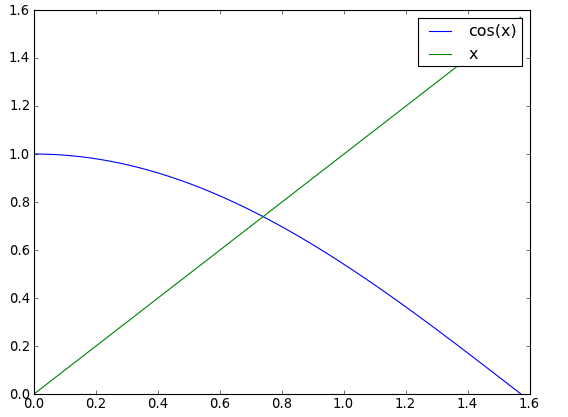
\includegraphics[width=0.8\textwidth]{imgp/xcosx.png}
\end{center}
\vspace{-2mm}
\caption{Graphs of the functions $\cos(x)$ and $x$ in the interval $(0, \pi/2)$.}
\label{fig:xcosx}
\end{figure}
\noindent
Looking at the graphs, clearly the solution is somewhere 
between $0.7$ and $0.8$. 
An engineer would not be extremely happy with such an answer though, 
so we need to make this guess more accurate. Looking at the graphs again, we can see
that in order to reach the intersection point, we can depart from zero and make very 
small steps to the right while the graph of $\cos(x)$ is above the graph of $x$.
Let's do this, and stop 
at the first point where $\cos(x)$ will be less than $x$. Our step will be called {\tt dx},
and our moving point on the $x$-axis will be called simply {\tt x}. We will also count 
steps via the variable {\tt n}. Choosing {\tt dx = 1e-6} will give us the result accurate 
to five decimal digits:

\begin{verbatim}
from numpy import cos
x = 0
dx = 1e-6
n = 0
while cos(x) > x:
    x += dx
    n += 1
print "Result is approximately", x
print "Steps made:", n
\end{verbatim}
Output:

\begin{verbatim}
Result is approximately 0.739086
Steps made: 739086
\end{verbatim}
In other words, the {\tt while} loop run 739086 times. Can you 
imagine doing this on your pocket calculator?

We should remark that the numerical method that we used was rather 
naive and in fact it took quite a bit of CPU time. Scientific computing
is an exciting field where researchers develop new methods that 
can solve problems like this more accurately and using less CPU time. 
In particular, for our problem there are much more powerful methods that can do the
same or better job using just five or six steps (!). One of them 
is the {\em Newton's method}. If you like what we did here, we encourage 
you to explore more math functionality and in particular numerical 
methods in NCLab. There are displayed projects for the Newton's method
and other methods to solve nonlinear equations and nonlinear equation systems.




\subsection{Programming exercises}

\begin{enumerate}
\item There is a jar of volume $V$ that is full of water. Every day, 
$P$ per cent of the water volume evaporates. Write a function 
{\tt water(V, P, R)} that prints the remaining water volume day
by day. The process stops when the volume is less than or equal to 
a residual volume $R$. Your function should return the number of 
days the process took. Include a condition at the beginning 
of the function that will output a warning and return zero 
if (a) $R > V$ or (b) $V <= 0$ or (c) $R <= 0$.
\item Imagine that you stand on a very high bridge $H$ meters above 
the river and throw a stone with velocity $v$ in horizontal direction. 
The coordinates of the flying stone as functions of time $t$ are
$x(t) = t v$ and $y(t) = H - 0.5gt^2$ where $g = 9.81$ kgms$^{-2}$ is
the gravitational acceleration. Use these formulas to write a function 
{\tt stone(t, H, v)} that for any time {\tt t} returns the $x$ and 
$y$ coordinates of the flying stone. Then calculate and plot the trajectory 
of the stone since the moment it leaves your hand until it falls into the 
river! Hint: Proceed by choosing a small time step {\tt dt} such 
as $0.01$ seconds, and use the function {\tt stone(t, H, v)} to generate 
a sequence of points for the {\tt plot()} command.  
\item The way Archimedes first estimated the value of $\pi$ was 
by taking a circle and calculating the perimeters of inscribed and 
circumscribed equilateral polygons with many edges. Let's do the same 
with the help of a computer! Proceed as follows: Choose some radius 
$R > 0$. Write a function {\tt in(R, n)} that will calculate the perimeter 
of an equilateral polygon with $n$ edges that is inscribed into the
circle of radius $R$. Then write a function {\tt out(R, n)}
that calculates the perimeter of a circumscribed equilateral polygon 
with $n$ edges. Choose a tolerance {\tt tol} such as {\tt 1e-3} and 
begin with $n = 3$. For each $n$ calculate the values {\tt in(R, n)}
and {\tt out(R, n)}. While the difference between these areas is 
greater than {\tt tol}, keep increasing $n$ by one. After the while 
loop finishes, take the final perimeters, divide them by $2 R$, and 
you just calculated a lower and upper estimate of $\pi$! 
\end{enumerate}


\section{Strings} \label{sec:strings}

\subsection{Objectives}

\begin{itemize}
\item Learn basic operations with single and multiline strings.
\item Learn to use quotes and backslashes, and to concatenate and repeat strings.
\item Learn to refer to letters by indices, parse strings, and slice them.
\end{itemize}
By a {\em string} we mean a text surrounded by double or single quotes, such as 
{\tt "this is a string"} or {\tt 'this is a string as well'}.
Strings are useful to make outputs more informative, but 
they have many other uses as well. For example, they can represent data 
in databases such as in a phone book. So we need to understand them well,
as well as various operations that we can do with them.

\subsection{Using quotes}

Let us first understand how to use quotes in strings. The safest way is to use 
them with a backslash:

\begin{verbatim}
print "I said \"yes\"."
\end{verbatim}
Output:

\begin{verbatim}
'I said "yes".'
\end{verbatim}
Another example:

\begin{verbatim}
print "It doesn\'t matter."
\end{verbatim}
Output:

\begin{verbatim}
"It doesn't matter."
\end{verbatim}

\subsection{Multiline strings and backslashes}

If we want to use multiline strings, the best way is to enclose them 
in triple quotes: 

\begin{verbatim}
edgar = """
Once upon a midnight dreary, while I pondered weak and weary,
Over many a quaint and curious volume of forgotten lore,
While I nodded, nearly napping, suddenly there came a tapping,
As of some one gently rapping, rapping at my chamber door.
`'Tis some visitor,' I muttered, `tapping at my chamber door -
Only this, and nothing more.'
"""
print edgar
\end{verbatim}
Output:

\begin{verbatim}

Once upon a midnight dreary, while I pondered weak and weary,
Over many a quaint and curious volume of forgotten lore,
While I nodded, nearly napping, suddenly there came a tapping,
As of some one gently rapping, rapping at my chamber door.
`'Tis some visitor,' I muttered, `tapping at my chamber door -
Only this, and nothing more.'

\end{verbatim}
Yes, there is one empty line on top and one on bottom. The reason is that 
Python inserted newline symbols there. If we want to avoid these empty lines, 
we have to include a backslash after the first triple quote, and also at the 
end of the last line before the closing triple quote. The backslash prevents 
Python from inserting a newline symbol into the string. Let us show one more 
example on backslashes. The string 

\begin{verbatim}
"""\
This is the first line,
and this is the second line.\
""" 
\end{verbatim}
will render as

\begin{verbatim}
'This is the first line,\nand this is the second line.' 
\end{verbatim}
When a backslash is included at the end of the first line of text,

\begin{verbatim}
"""\
This is the first line,\
and this is the second line.\
""" 
\end{verbatim}
we obtain 

\begin{verbatim}
'This is the first line,and this is the second line.'
\end{verbatim}
Yes we need to watch for empty characters! Inserting one before the second 
backslash,

\begin{verbatim}
"""\
This is the first line, \
and this is the second line.\
""" 
\end{verbatim}
we finally obtain 

\begin{verbatim}
'This is the first line, and this is the second line.'
\end{verbatim}


\subsection{Concatenation and repetition}

Strings can be concatenated (glued together) with the '{\tt +}' operator, and repeated with '{\tt *}':

\begin{verbatim}
word = 'Help' + 'me!'
print "I yelled" + 3 * word
\end{verbatim}
Output:

\begin{verbatim}
I yelledHelpme!Helpme!Helpme!
\end{verbatim}
You can see that empty spaces matter. Let's try again:

\begin{verbatim}
word = '\"Help' + ' me!\" '
print "I yelled " + 3 * word
\end{verbatim}
Output:

\begin{verbatim}
I yelled "Help me!" "Help me!" "Help me!"
\end{verbatim}

\subsection{Referring to letters by their indices}\label{subsec:ind}

Individual letters forming a string can be accessed via indices. The indices 
start from zero. It is also handy to use the index {\tt -1} 
for the last index, {\tt -2} for the one-before-last etc.

\begin{verbatim}
word = "breakfast"
print "First character:", word[0]
print "Second character:", word[1]
print "Last character:", word[-1]
print "One-before-last character:", word[-2]
\end{verbatim}
Output:

\begin{verbatim}
First character: b
Second character: r
Last character: t
One-before-last character: s
\end{verbatim}

\subsection{Parsing strings with the {\tt for} loop}\label{subsec:forstr} 

The length of a string is obtained using the function {\tt len()}.
Example:

\begin{verbatim}
word = "breakfast"
n = len(word)
print "Length of the string:", n
\end{verbatim}
Output:

\begin{verbatim}
Length of the string: 9
\end{verbatim}
In order to parse strings, it is practical to introduce the Python counting 
({\tt for}) loop. We do this ahead of time, more on the {\tt for} loop will 
be said in Section \ref{sec:forloop}. Let us begin with an example again: The
following code parses the string {\tt word} letter by letter and prints all
the letters:

\begin{verbatim}
word = "breakfast"
n = len(word)
for i in range(n):
    print word[i]
\end{verbatim}
Output:

\begin{verbatim}
b
r
e
a
k
f
a
s
t
\end{verbatim}
This deserves some explanation. Calling the function {\tt range(n)} generates 
a sequence of integers that goes from zero to {\tt n-1}. Let's try this:

\begin{verbatim}
print range(3)
\end{verbatim}
Output:

\begin{verbatim}
[0, 1, 2]
\end{verbatim}
Another example:

\begin{verbatim}
print range(10)
\end{verbatim}
Output:

\begin{verbatim}
[0, 1, 2, 3, 4, 5, 6, 7, 8, 9]
\end{verbatim}
When called with two arguments, {\tt range(n1, n2)} will generate 
a sequence {\tt [n1, n1+1, n1+2, ..., n2-1]}. Example:

\begin{verbatim}
print range(4, 10)
\end{verbatim}
Output:

\begin{verbatim}
[4, 5, 6, 7, 8, 9]
\end{verbatim}
The {\tt for} loop goes through the sequence generated by the {\tt range()} function, 
taking one element per cycle. So in the first cycle, the variable {\tt i}
has the value {\tt 0}, in the second cycle {\tt i} is {\tt 1}, in the third cycle 
{\tt i} is {\tt 2} etc., until the end of the sequence is reached. 

Since we know from Subsection \ref{subsec:ind} 
how to index letters in a string via their indices, now the above 
code that decomposed the word {\tt breakfast} into individual letters
makes perfect sense!

\subsection{Slicing strings}

We can also access substrings, this is called {\em slicing}:

\begin{verbatim}
w1 = "bicycle"
w2 = w1[0:3]
print w2
\end{verbatim}
Output:

\begin{verbatim}
bic
\end{verbatim}
An omitted first index in a slice defaults to zero:

\begin{verbatim}
w3 = w1[0:2]
print w3
\end{verbatim}
Output:

\begin{verbatim}
bi
\end{verbatim}
An omitted second index defaults to the length of the string:

\begin{verbatim}
w4 = w1[2:]
print w4
\end{verbatim}
Output:

\begin{verbatim}
cycle
\end{verbatim}
This is enough for now but hold on -- many wonderful operations one 
can do with text strings will be shown in Subsection \ref{subsec:textstrclass}



\subsection{Programming exercises}

\begin{enumerate}
\item Write a function {\tt countchars(str, L)} that will count 
all occurences of the character (one-letter string) {\tt L} in the string {\tt str}, 
and return their number. 
\item Write a function {\tt countwords(str, word)} that will count 
all occurences of the string {\tt word} in the string {\tt str}, and 
return their number. You can assume that {\tt len(str)} is always greater 
or equal to {\tt len(word)}.
\item Write a function {\tt searchandreplace(str, word1, word2)} that will 
find all occurences of the string {\tt word1} in the string {\tt str}, and 
replace them with the string {\tt word2}. Return the new string.
Hint: Do not replace in the existing string {\tt str} - instead, 
create a new string {\tt str2} and add into it what is needed.
\end{enumerate}



\section{Tuples, Lists, and Dictionaries}\label{sec:lists}

\subsection{Objectives}

\begin{itemize}
\item Learn to store data in tuples, lists, and dictionaries.
\item Learn basic differences between these data types, and their best use cases.
\item Learn useful built-in functions to operate with these data structures efficiently. 
\end{itemize}
Tuples, lists, and dictionaries belong to the most important data structures in Python, and the 
language offers a wide range of functionality to work with them efficiently. They become 
especially useful in combination with the {\tt for}
loop that was already mentioned in Subsection \ref{subsec:forstr}, and that will be 
discussed in more detail in Section \ref{sec:forloop}. 

\subsection{Tuples}

Let us begin with tuples. Tuples are perfect for sequences 
of data that does not change in time - such as 
the names of weekdays, or names of months. To define a tuple, 
enclose comma-separated items in round brackets:

\begin{verbatim}
months = ('January', 'February', 'March', 'April', 'May', 'June',\
'July', 'August', 'September', 'October', 'November', 'December')
\end{verbatim}
The items in the tuple {\tt months} are all strings, but they do not
have to be. A tuple can be very heterogeneous -- it can contain strings,
numbers, other tuples, etc. Although -- in simplicity is beauty, we
do not have to always take advantage of the extreme possibilities.
It is important to remember that {\bf a tuple, once defined, cannot 
be changed} in the sense that no new items can be added and existing 
items cannot be deleted.

Items in a tuple are referenced by indices, in the same way as individual 
characters are referenced in a text string. Remember that indices always 
start from zero:

\begin{verbatim}
print "First month:", months[0]
print "Second month:", months[1]
print "Third month:", months[2]
\end{verbatim}
Output:

\begin{verbatim}
First month: January
Second month: February
Third month: March
\end{verbatim}
Index {\tt -1} refers to the last item, {\tt -2} to the one before last, etc.:

\begin{verbatim}
print "One before last month:", months[-2]
print "Last month:", months[-1]
\end{verbatim}
Output:

\begin{verbatim}
One before last month: November
Last month: December
\end{verbatim}

\noindent
We can {\em slice} tuples similarly to how we sliced strings:

\begin{verbatim}
months[2:5]
\end{verbatim}
Output:

\begin{verbatim}
('March', 'April', 'May')
\end{verbatim}
The length of a tuple is obtained using the function {\tt len()}:

\begin{verbatim}
len(months)
\end{verbatim}
Output:

\begin{verbatim}
12
\end{verbatim}

\subsection{Lists}

Lists are similar to tuples, and all indexing and slicing works in the same way. 
Empty list {\tt L} is defined as follows:

\begin{verbatim}
L = []
\end{verbatim}
The biggest difference between a tuple 
and a list is that {\bf items in a list can be changed}. So, we use
lists for items that can change in time. Let's say that there are 
10 people in a school class {\tt cls}:

\begin{verbatim}
cls = ['John', 'Pam', 'Emily', 'Jessie', 'Brian', \
'Sam', 'Jim', 'Tom', 'Jerry', 'Alex']
\end{verbatim}
Then however, Emily moves to a different city:

\begin{verbatim}
del cls[2]
print cls
\end{verbatim}
Output

\begin{verbatim}
['John', 'Pam', 'Jessie', 'Brian', 'Sam', 'Jim', 
'Tom', 'Jerry', 'Alex']
\end{verbatim}
After some time, a new student Jack moves in:

\begin{verbatim}
cls.append('Jack')
print cls
\end{verbatim}
Output

\begin{verbatim}
['John', 'Pam', 'Jessie', 'Brian', 'Sam', 'Jim', 
'Tom', 'Jerry', 'Alex', 'Jack']
\end{verbatim}
Useful can be the function {\tt pop()} that deletes an item and returns it for further
use (as opposed to {\tt del} which just deletes the item):

\begin{verbatim}
name = cls.pop(2)
print name 
print cls
\end{verbatim}
Output

\begin{verbatim}
Jessie
['John', 'Pam', 'Brian', 'Sam', 'Jim', 
'Tom', 'Jerry', 'Alex', 'Jack']
\end{verbatim}
New item can be inserted at an arbitrary position using the function {\tt insert()}:

\begin{verbatim}
cls.insert(3, 'Daniel')
print cls
\end{verbatim}
Output:

\begin{verbatim}
['John', 'Pam', 'Brian', 'Daniel', 'Sam', 'Jim', 
'Tom', 'Jerry', 'Alex', 'Jack']
\end{verbatim}
A list can be sorted via the function {\tt sort()}:

\begin{verbatim}
cls.sort()
print cls
\end{verbatim}
Output:

\begin{verbatim}
['Alex', 'Brian', 'Daniel', 'Jack', 
'Jerry', 'Jim', 'John', 'Pam', 'Sam', 'Tom']
\end{verbatim}
The function {\tt reverse()} reverses a list:

\begin{verbatim}
cls.reverse()
print cls
\end{verbatim}
Output:

\begin{verbatim}
['Tom', 'Sam', 'Pam', 'John', 'Jim', 
'Jerry', 'Jack', 'Daniel', 'Brian', 'Alex']
\end{verbatim}
The function {\tt count()} counts the number of occurences of an item
in the list:

\begin{verbatim}
cls.count('Jerry')
\end{verbatim}
Output:

\begin{verbatim}
1
\end{verbatim}
The function {\tt index()} returns the index of the first occurence 
of an item. If the item is not found, error is thrown:

\begin{verbatim}
cls.index('Jerry')
\end{verbatim}
Output:

\begin{verbatim}
5
\end{verbatim}
Another useful operation with lists is their {\em zipping}. The {\tt zip} command takes two lists as arguments 
and creates a new list of pairs. Example:

\begin{verbatim}
A = [1, 2, 3]
B = ['x', 'y', 'z']
print zip(A, B)
\end{verbatim}
Output:

\begin{verbatim}
[(1, 'x'), (2, 'y'), (3, 'z')]
\end{verbatim}
If the lists are not equally-long, the superfluous items in the longer list 
are skipped:

\begin{verbatim}
A = [1, 2, 3, 4, 5]
B = ['x', 'y', 'z']
print zip(A, B)
\end{verbatim}
Output:

\begin{verbatim}
[(1, 'x'), (2, 'y'), (3, 'z')]
\end{verbatim}

\subsection{Dictionaries}

Sometimes we need to store additional information for 
people (or general items) in a list. Such information may be  
their phone number, age, weight, address, family 
status and/or many other things. In this context, the 
people's names are said to be {\em keys} and the additional 
information are the corresponding {\em values}. Of course this 
is not only about people, we can have a list of cars and the 
additional information to each car may be its price, mileage, or
gas consumption. And we should not forget to mention a real 
dictionary, where the keys can be English words and the values the 
corresponding Spanish translations.

The data structure containing keys and values is called a {\em dictionary}. 
An empty dictionary {\tt D} is defined as follows:

\begin{verbatim}
D = {}
\end{verbatim}
An example of a phone book would be:

\begin{verbatim}
phonebook = {'Peter Parson': 8806336, 'Emily Everett': 6784346, \
'Lewis Lame': 1122345}
\end{verbatim}
{\bf Note the curly brackets.} 
Once we have created a new phone book, we may want to add a new person to it:

\begin{verbatim}
phonebook['Silly Sam'] = 1234567
print phonebook
\end{verbatim}
Output:

\begin{verbatim}
{'Peter Parson': 8806336, 'Emily Everett': 6784346,
'Lewis Lame': 1122345, 'Silly Sam': 1234567}
\end{verbatim}
And we can also delete a person from the phonebook:

\begin{verbatim}
del phonebook['Peter Parson']
print phonebook
\end{verbatim}
Output:

\begin{verbatim}
{'Emily Everett': 6784346, 'Lewis Lame': 1122345, 
'Silly Sam': 1234567}
\end{verbatim}
We can check if a key is in the dictionary:

\begin{verbatim}
if phonebook.has_key('Silly Sam'):
    print "Silly Sam's phone number is", phonebook['Silly Sam']
else:
    print "Silly Sam is not in the phonebook."
\end{verbatim}
Output:

\begin{verbatim}
Silly Sam's phone number is 1234567
\end{verbatim}
To get the list of all keys, we type:

\begin{verbatim}
phonebook.keys()
\end{verbatim}
Output:

\begin{verbatim}
['Emily Everett', 'Lewis Lame', 'Silly Sam']
\end{verbatim}
Similarly, we can also get the list of all values:

\begin{verbatim}
phonebook.values()
\end{verbatim}
Output:

\begin{verbatim}
[6784346, 1122345, 1234567]
\end{verbatim}
It is important to remember that {\bf dictionaries are not ordered} in any 
special way. While a list can be sorted, a dictionary can not. They are only 
designed to get you the value for a given key. 
The length of a dictionary can be obtained using the function {\tt len()}:

\begin{verbatim}
len(phonebook)
\end{verbatim}
Output:

\begin{verbatim}
3
\end{verbatim}
There are additional functions that one can use with dictionaries. However, 
what we mentioned so far is enough for an introductory course and we refer 
to the Python tutorial\footnote{http://docs.python.org/tutorial} for more 
details.


\subsection{Programming exercises}

\begin{enumerate}
\item Write a Python function {\tt select(T, n)} that for any tuple {\tt T}
      returns its item with index {\tt n}. Indices start from zero as usual.
      If index is out of range, print "Index out of range, returning zero." and 
      return zero.
\item Write a Python function {\tt supersort(LL)} that takes a list of lists {\tt LL}, 
      rearranges the order of lists in {\tt LL} according to their length increasingly,
      and returns the sorted list of lists. 
\item Write a Python function {\tt sortdict(D, n)} where {\tt D} is a dictionary whose values 
      are lists. For an index {\tt n}, your function should return the list of keys sorted 
      according to the values with index {\tt n}, in increasing order. 
\end{enumerate}

\section{The {\tt for} Loop} \label{sec:forloop}

\subsection{Objectives}

\begin{itemize}
\item Review the {\tt range()} function and understand that it creates a Python list.
\item Understand when the Python {\tt for} loop should be used.
\item Learn that the {\tt for} loop can go over any list or tuple.
\end{itemize}
Before we bring up the {\tt for} loop, let us revisit the {\tt range()}
function that was first mentioned in Section \ref{sec:strings}. After 
learning about tuples, lists and dictionaries in Section \ref{sec:lists}, the 
reader will not be surprized when we state that this function produces 
a Python list of integer numbers. For example:

\begin{verbatim}
range(10)
\end{verbatim}
produces the following output:

\begin{verbatim}
[0, 1, 2, 3, 4, 5, 6, 7, 8, 9]
\end{verbatim}
It is possible to start from a different number:

\begin{verbatim}
range(3, 10)
\end{verbatim}
Output:

\begin{verbatim}
[3, 4, 5, 6, 7, 8, 9]
\end{verbatim}
The {\tt for} loop in Python is a {\em counting loop} analogous to the {\tt repeat}
loop in Karel the Robot. Thus it should be used when we know how many repetitions there 
will be. However, in Python, the counting loop is not restricted to integer numbers 
only. It is much more general -- {\em it goes over the items of aa arbitrary list or tuple}. 

\subsection{Combined with the {\tt range()} function}

When used in combination with the {\tt range()} function, it goes over integer indices. 
Example:

\begin{verbatim}
for i in range(10):
    print i
\end{verbatim}
Output:

\begin{verbatim}
0
1
2
3
4
5
6
7
8
9
\end{verbatim}
As usual, note indentation of the body of the loop, which has the same 
purpose as indentation in the {\tt while} loop. 

\subsection{Combined with a general list or tuple}

Remember our tuple of months? We can use the {\tt for} loop to print them as well:

\begin{verbatim}
for m in months:
    print m
\end{verbatim}
Output:

\begin{verbatim}
January
February
March
April
May
June
July
August
September
October
November
December
\end{verbatim}
The {\tt for} loop works in the same way with lists -- it does not distinguish between these 
two data types at all.

\subsection{Reverting a dictionary}

Remember that it is easy to extract keys and values from a dictionary using the 
{\tt keys()} and {\tt values()} functions? In either case, the result of this operation 
is a {\em Python list}, which in turn can be used with the {\tt for} loop. That was easy. Let us do something more interesting -- 
perhaps convert an English-Spanish dictionary into a Spanish-English one? 

\begin{verbatim}
ES = {'city': 'ciudad', 'fire': 'fuego', 'sun': 'sol'}
SE = {}
for english_word in D:
    spanish_word = D[english_word]
    SE[spanish_word] = english_word
    
print "Spanish-English dictionary:"
print SE
\end{verbatim}
The output of this program is:

\begin{verbatim}
Spanish-English dictionary:
{'ciudad': 'city', 'sol': 'sun', 'fuego': 'fire'}
\end{verbatim}
Isn't Python beautifully simple?



\subsection{Programming exercises}

\begin{enumerate}
\item Write a Python function {\tt primes(n)} that for a positive number {\tt n} returns the list 
      of all prime numbers that are less than or equal to {\tt n}. The list 
      should be sorted increasingly. Remember that the smallest prime number is 2.
\item Write a Python function {\tt charstats(L)} that takes a list of 
      text strings {\tt L}, and creates a statistics of characters present in {\tt L}. 
      The text strings in {\tt L} can contain alphabetic, numeric, and special characters. 
      Your function should return a dictionary whose keys are the different characters. 
      For each character in the dictionary, the value is the number of its appearances 
      in {\tt L}.
\item The Rubik's cube shown in Fig. \ref{fig:rubik} is a famous brain teaser. Initially,
      each face has nine fields of the same color, and there are six different colors on the 
      cube (one per each face).
      The cube has three layers in each axial direction that can rotate about the axis.
      Your task is to implement a Python function {\tt rubik()} that calculates the total 
      number of all possible states of the cube
      accounting for different rotations (in other words, rotating the entire 
      cube by 90 degrees in any of the three axial directions yields a different state).

\begin{figure}[!ht]
\begin{center}
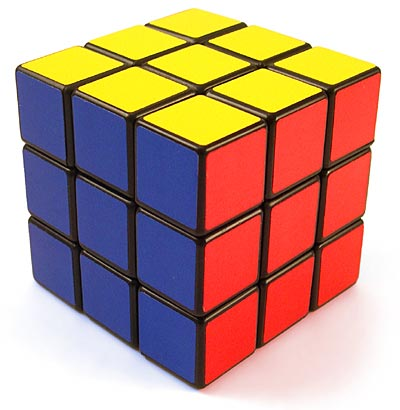
\includegraphics[width=0.4\textwidth]{imgp/rubix_cube.jpg}
\end{center}
\vspace{-2mm}
\caption{Rubik's cube.}
\label{fig:rubik}
\end{figure}
\noindent

\item Write a Python function {\tt maximize(L1, L2)} that takes two lists of real numbers and 
finds a number {\tt n1} in {\tt L1} and a number {\tt n2} in {\tt L2} such that the product 
{\tt n1 * n2} is maximal. Return the numbers {\tt n1} and {\tt n2}.

\end{enumerate}

\section{Catching and Raising Exceptions}

\subsection{Objectives}

\begin{itemize}
\item Understand what exceptions are, when they can occur, and how to catch them.
\item Learn to never underestimate the user.
\item Understand {\tt ZeroDivisionError} and other exceptions.
\item Learn to use the {\tt assert()} function and catch the {\tt AssertionError} exception.
\item Learn how to raise exceptions using the {\tt raise} statement.
\end{itemize}
Imagine that you have to write a Python function to evaluate
$$
f(x) = \frac{1}{9 - x^2}.
$$
Of course, this is simple!

\begin{verbatim}
def f(x):
    return 1. / (9 - x**2)
\end{verbatim}
But we can almost guarantee that the first user will call the 
function with $x = 3$ or $x = -3$. What does he see?

\begin{verbatim}
Traceback (most recent call last):
  File "<nclab>", line 1, in <module>
ZeroDivisionError: float division by zero
\end{verbatim}

\subsection{Never underestimate the user}

We need to be very careful with users! If we are not, they always manage
to crash our code. By always we mean {\em always}. And most often they do even
if we are as careful as possible. Sometimes they do it for fun, to show us that we are not all that smart.
But most of the time they do it without bad intentions -- they are just learning to use our
program, not knowing what they are not supposed to do, stepping over boundaries that we would 
never cross. For example, the author of the function 

\begin{verbatim}
from numpy import sqrt
def invsqrt(x):
    return 1./sqrt(x)
\end{verbatim}
would hardly call it with {\tt x = 0}, or even {\tt x = -1}. {\em The function 
was not designed for that!} But the user did not know it.

Here is an alternative version of the above function {\tt f(x)} that will not crash:

\begin{verbatim}
def f(x):
    if x != 3 and x != -3:
        return 1. / (9 - x**2)
    else:
        print "Division by zero detected, returning 0."
        return 0
\end{verbatim}
However, it is useful to slow down here and look at what we have. The fact that
the warning sentence is printed is not very useful, because it is printed as output for 
the human eye only. What if there is nobody to read it? Even if division by zero 
happens, the function returns zero (a valid number) and the program continues on.
Not good. Fortunately,
Python (and other languages) have an elegant way to take care of exceptional situations 
like this. This is called {\em exceptions handling}.

\subsection{{\tt ZeroDivisionError} Exception}

In contrast 
to {\em predicting} what possibily could go wrong and including conditions to detect wrong 
input, we do not check the input and let it simply happen. Does it sound careless? Let us 
return to the original simple form of the function {\tt f(x)}:

\begin{verbatim}
def f(x):
    return 1. / (9 - x**2)
\end{verbatim}
This is the function that we will use. However, we will call it in such a way that 
an exceptional situation (here division by zero) is captured. For this we use the 
{\tt try} command:
 
\begin{verbatim}
try:
    result = f(a)
except ZeroDivisionError:
    print "Division by zero detected, performing emergency scenario!"
else:
    print "Evaluation of f(a) was successful, going on normally."
\end{verbatim}
Before continuing, we recommend that you type this code into the code cell,
including the definition of the function {\tt f(x)}, and run it with values
that crash the function {\tt f(x)} and with values that do not. If you are a newcomer to
exceptions, this is an interesting experience. Feels a bit like letting the
airplane crash, but save all passengers afterwards.
 
\subsection{The {\tt assert()} function}

The {\tt assert()} function raises an exception whenever the Boolean 
statement used as its argument is {\tt False}. This is a powerful tool to raise our own 
exceptions. These exceptions can be caught using the {\tt try} command 
as all other exceptions:

\begin{verbatim}
def f(x):
    assert(x != 3 and x != -3)
    return 1. / (9 - x**2)

try:
    result = f(a)
except AssertionError:
    print "Assertion failed, performing emergency scenario!"
else:
    print "Assertion passed, going on normally."
\end{verbatim}
When called with {\tt a} equal to {\tt 1}, this code gives:

\begin{verbatim}
Assertion passed, going on normally.
\end{verbatim}
When called with {\tt a} equal to {\tt 3}, this is what happens:

\begin{verbatim}
Assertion failed, performing emergency scenario!
\end{verbatim}

\subsection{The {\tt raise} statement}

Python does not have a command to stop program execution. Sometimes this is
need though, such as when the user calls our function with incorrect data. 
To illustrate this, let us return to the function {\tt invsqrt()} that was 
defined above, but now we include a {\tt raise} command in it:
 
\begin{verbatim}
from numpy import sqrt
def invsqrt(x):
    if x <= 0:
      raise ValueError("Please do not call the invsqrt() \
function when x is zero or negative.")
    return 1./sqrt(x)
\end{verbatim}
Now the output of {\tt invsqrt(-5)} is:

\begin{verbatim}
Traceback (most recent call last):
  File "<string>", line 1, in <module>
  File "<nclab>", line 4, in invsqrt
ValueError: Please do not call the invsqrt() 
function when x is zero or negative.
\end{verbatim}
Incorrect values of user input are the most common cause for raising 
exceptions on our own. Any other exception type can be raised as well
if needed.

\subsection{Other types of exceptions}

There are many different exceptions including {\tt MemoryError} (program runs out of memory),
{\tt NameError} (local or global name is not found), {\tt OverflowError} (result of an arithmetic 
operation is too large to be represented), {\tt SyntaxError} (parser encounters a syntax error),
{\tt IndentationError} (parser finds incorrect indentation), {\tt UnboundLocalError} (reference 
is made to a local variable in a function or method, but no value has been bound to that variable),
and others. All of them can be caught using the {\tt try} command. If you are interested in 
learning more, visit http://docs.python.org/library/exceptions.html.



\subsection{Programming exercises}

\begin{enumerate}
\item Implement a custom plotting function {\tt sureplot(f, a, b, label, n = 100)} where {\tt f(x)} is 
      a user-supplied real function, {\tt (a, b)} is an interval, {\tt label} 
      is a text string label for the plot, and {\tt n} is the plotting subdivision of the interval {\tt (a, b)}.
      Implement exception handling in such a way that if the user's function is not defined for some {\tt x}, 
      a warning is printed and the corresponding point is not added to the plot. But the rest of the graph
      will be plotted normally. For example, if the use wants to plot the function 
\begin{verbatim}
def f(x):
    return log(x)
\end{verbatim}
in the interval {\tt (-1, 1)} then the left half of the graph will be missing but the rest 
will be displayed correctly.
\item Implement a Boolean function {\tt dryrun(f)} which will run any user-supplied function {\tt f()}.
      If the function {\tt f()} contains a syntax error, print a warning and return {\tt False}. If the 
      call to the user's function was successful, return {\tt True}.
\end{enumerate}

\section{Object-Oriented Programming}

\subsection{Objectives}

\begin{itemize}
\item Understand the philosophy of object-oriented (OO) programming.
\item Understand the difference between OO programming and procedural programming.
\item Learn basic concepts -- classes, objects, and methods.
\item Learn the syntax of defining and instantiating classes in Python.
\end{itemize}
Since the very beginning of this course, 
we have put emphasis on designing simple algorithms
and writing clean, transparent code. This included:
\begin{itemize}
\item Creating custom functions for functionality that can be reused.
\item Keeping all variables as local as possible
\end{itemize}
Object-oriented programming brings these good programming practices to
perfection -- it will help us to write crystal clear, elegant, and very safe code.

\subsection{From procedural to object-oriented programming}

The programming style we have been using so far is called {\em procedural programming}.
The name, of course, comes from using {\em procedures} to solve various tasks that 
lead to the solution of the problem at hand. Procedure is an activity, a sequence of operations 
done with data that is supplied to it. {\em Procedures do not own the data they 
operate with.} 

This, however, means that the data must be stored somewhere else. In other
words, the range of validity of the data extends beyong the borders of the 
function where it is processed. 
Can you see an analogy to using local and global variables? It is great
to keep variables local, and in the same way it would be great to make
data local to procedures that operate with them. But wait, this is called {\em 
object-oriented programming!}

\subsection{Example: Moving to a different city}

Here is a real-life example demonstrating the difference between 
procedural and object-oriented programming. Imagine that you are moving 
and all your things need to be packed, boxed, loaded on a truck, hauled 
a 1000 miles, unloaded, and brought into your new home. 

{\em Procedural approach:} You (the procedure) 
go rent a truck -- this is the data that the procedure does not own. Then
you pack everything, load it on the truck, drive to the other city, 
unload your things, and carry them into your new home. Then you go 
return the truck (that's the return statement at the end of the procedure).

{\em Object-oriented approach:} You call a moving company "C". This means 
that you just created an object C. Note that the 
object C owns the truck. They will come to your home and use methods 
C.pack(), C.box(), C.load(), C.haul(), C.unload(), C.carry() and perhaps 
even C.unpack() to solve your problem. Notice the following benefits of the object-oriented approach: 
\begin{itemize}
\item The work is being done by the company, 
      you do not have to worry (delegation of work).
\item You do not have to be able to drive a truck (better code structure). 
\item You do not need to know how the company does the moving (reduced flow of data).
\item You can concentrate on solving problems 
      in your area of expertise (greater efficiency).
\item You do not risk crashing the truck (safer programming).
\end{itemize}

\subsection{Classes, objects, and methods}

Let us stay with the moving example for a little while longer. The moving 
company that you heard of, or that you saw in an advertisement, 
is a {\em class} or in other words a {\em concept}. Formally, we say that 
{\em class} is an entity comprising data and functionality that uses the data.
But a concept will not get your things moved. For that you need a concrete team of 
movers. This is called an {\em object} or an {\em instance of the class}. 

When the movers appear at your doorstep, that's when an instance 
of the class is created. When they pack, box, and load your things, the object is using 
{\em methods} of the class. Technically, methods belong to the class because that's
where they are defined, but often we say that ``an objects uses its methods to ...". 
Once again, methods are {\em defined in a class} but {\em used 
by instances of the class}. 
Methods of a class can operate on data owned by the class (the truck) as well as 
on data that does not belong to the class (your things that are being moved.

Similarly with variables -- variables are defined in a class, but they do not 
have concrete values there. In the class definition, they are part of a concept. 
Only after an instance of the class is created, the variables are filled with 
concrete values. 

\subsection{An example from geometry}

Let's see how all this is implemented in Python. We will say goodbye to the movers
and play with some simple geometrical concepts instead. Let us create a class
{\tt circle}. The data owned by this class will be:

\begin{itemize}
\item Radius {\tt R}, 
\item center with coordinates {\tt Cx, Cy}, 
\item two arrays {\tt ptsx}, {\tt ptsy} to plot the circle. 
\end{itemize}
The methods of this class will include 
\begin{itemize}
\item {\tt \_\_init\_\_(self, r, cx, cy)} ... constructor,
\item {\tt area(self)} ... calculate and return its area,
\item {\tt perimeter(self)} ... calculate and return its perimeter,
\item {\tt draw(self)} ... draw itself.
\end{itemize}
Do not be disturbed by the funny way the constructor {\tt \_\_init\_\_} 
is defined in Python, or by the argument {\tt self} that is present 
in all methods. Constructors are 
used in all object-oriented languages to pass external parameters 
(such as the radius and the center point in this case) into newly 
created instances. In other words, each instance of the class {\tt circle} 
can have a different radius and a different center.

The keyword {\tt self} must be included in each method of the class 
and this is a reference to the concrete instance through which all
data and methods of the instance are accessed. Such a reference is present 
in other object-oriented languages as well - including C++ where the programmer
does not have to mention it explicitly like in Python. It is added there by 
the compiler.

\subsection{Defining and using class {\tt circle}} \label{subsec:circle}

This is how the class {\tt circle} is defined in Python:

\begin{verbatim}
from numpy import pi, cos, sin
from pylab import clf, plot, legend, axis

class circle:
    # Constructor:
    def __init__(self, r, cx, cy, n = 100):
        self.R = r
        self.Cx = cx
        self.Cy = cy
        self.n = n
        # And now the points for plotting:
        self.ptsx = []
        self.ptsy = []
        da = 2*pi/self.n
        for i in range(n):
            self.ptsx.append(self.Cx + self.R * cos(i * da))
            self.ptsy.append(self.Cy + self.R * sin(i * da))
        self.ptsx.append(self.Cx + self.R)
        self.ptsy.append(self.Cy + 0)
            
    # Method to return circle area:
    def area(self):
        return pi * self.R**2
      
    # Method to return perimeter:
    def perimeter(self):
        return 2 * pi * self.R
      
    # Method to plot the circle:
    def draw(self, label):
        axis('equal')
        plot(self.ptsx, self.ptsy, label = label)
        legend()
\end{verbatim}
Notice how the variables owned by the class are always used with the 
prefix {\tt self}.

With such a nice class in hand, it is easy to draw various circles,
and calculate their areas and perimeters:
\begin{verbatim}        
# Create an instance:
C1 = circle(1, 0, 0)
print "Are and perimeter of circle 1:", \
C1.area(), C1.perimeter()
C2 = circle(0.5, 1, 0)
print "Are and perimeter of circle 2:", \
C2.area(), C2.perimeter()
C3 = circle(0.25, 1.5, 0)
print "Are and perimeter of circle 3:", \
C3.area(), C3.perimeter()
clf()
C1.draw("First circle")
C2.draw("Second circle")
C3.draw("Third circle")
lab.show()
\end{verbatim}
The output (text and Fig. \ref{fig:3circ}) is shown below.

\begin{verbatim}
Area and perimeter of circle 1: 3.14159265359 6.28318530718
Area and perimeter of circle 2: 0.785398163397 3.14159265359
Area and perimeter of circle 3: 0.196349540849 1.57079632679
\end{verbatim}

\begin{figure}[!ht]
\begin{center}
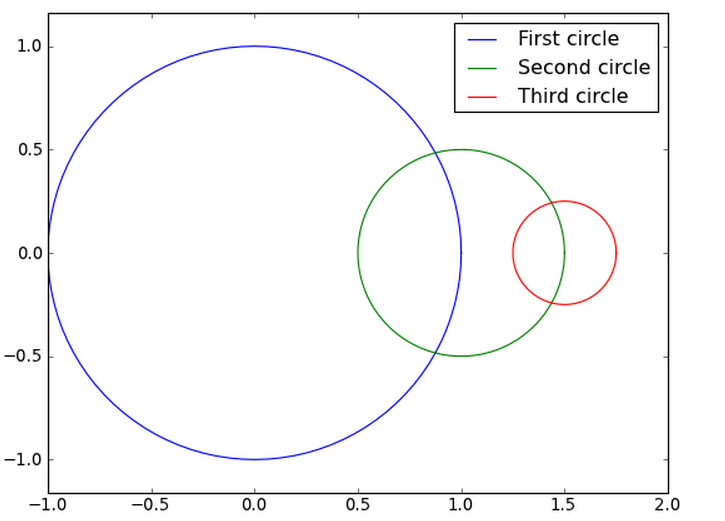
\includegraphics[width=0.8\textwidth]{imgp/3circ.png}
\end{center}
\vspace{-2mm}
\caption{Three instances of the class {\tt circle}.}
\label{fig:3circ}
\end{figure}

\subsection{Text string as a class} \label{subsec:textstrclass}

We first met text strings in Section \ref{sec:strings}. Now that 
we know how classes are defined and used, we can reveal that 
text string is a class! In fact it has many great methods that 
really make working with texts easy and fun. Let us show some 
of them. Below, arguments enclosed in brackets are optional,
and if they are used, then without the brackets:\\

\noindent
{\bf Method} {\tt capitalize()}\\

\noindent
Return a copy of the string with only its first character capitalized.\\

\noindent
\underline{Example}:
\begin{verbatim}
str = "sentences should start with a capital letter."
print str.capitalize()
\end{verbatim}
\underline{Output}:
\begin{verbatim}
Sentences should start with a capital letter.
\end{verbatim}
\vspace{4mm}

\noindent
{\bf Method} {\tt count(sub[, start[, end]])}\\

\noindent
Return the number of occurrences of substring sub in string S[start:end]. 
Optional arguments start and end are interpreted as in slice notation.\\

\noindent
\underline{Example}:
\begin{verbatim}
str = "John Stevenson, John Lennon, and John Wayne."
print str.count("John")
\end{verbatim}
\underline{Output}:
\begin{verbatim}
3
\end{verbatim}
\vspace{4mm}

\noindent
{\bf Method} {\tt find(sub[, start[, end]])}\\

\noindent
Return the lowest index in the string where substring {\tt sub} is found, such that 
sub is contained in the range {\tt [start, end]}. Optional arguments {\tt start} and {\tt end} 
are interpreted as in slice notation. Return {\tt -1} if {\tt sub} is not found.\\

\noindent
\underline{Example}:
\begin{verbatim}
str = "This happened during the summer."
print str.find("sum")
\end{verbatim}
\underline{Output}:
\begin{verbatim}
25
\end{verbatim}
\vspace{4mm}

\noindent
{\bf Method} {\tt index(sub[, start[, end]])}\\

\noindent
Like find(), but raise ValueError when the substring is not found.\\

\noindent
{\bf Method} {\tt isalnum()}\\

\noindent
Return true if all characters in the string are alphanumeric and 
there is at least one character, false otherwise.\\

\noindent
\underline{Example}:
\begin{verbatim}
str1 = "mypassword123"
if str1.isalnum():
    print str1, "is alphanumeric."
else: 
    print str1, "is not alphanumeric."
str2 = "mypassword123+"
if str2.isalnum():
    print str2, "is alphanumeric."
else: 
    print str2, "is not alphanumeric."
\end{verbatim}
\underline{Output}:
\begin{verbatim}
mypassword123 is alphanumeric.
mypassword123+ is not alphanumeric.
\end{verbatim}
\vspace{4mm}

\noindent
{\bf Method} {\tt isalpha()}\\

\noindent
Return true if all characters in the string are alphabetic and 
there is at least one character, false otherwise.\\

\noindent
\underline{Example}:
\begin{verbatim}
str1 = "John"
if str1.isalpha():
    print str1, "is alphabetic."
else: 
    print str1, "is not alphabetic."
str2 = "My name is John"
if str2.isalpha():
    print str2, "is alphabetic."
else: 
    print str2, "is not alphabetic."
\end{verbatim}
\underline{Output}:
\begin{verbatim}
John is alphabetic.
My name is John is not alphabetic.
\end{verbatim}
\vspace{4mm}

\noindent
{\bf Method} {\tt isdigit()}\\

\noindent
Return true if all characters in the string are digits and there is at least one character, false otherwise.\\

\noindent
\underline{Example}:
\begin{verbatim}
str1 = "2012"
if str1.isdigit():
    print str1, "is a number."
else: 
    print str1, "is not a number."
str2 = "Year 2012"
if str2.isdigit():
    print str2, "is a number."
else: 
    print str2, "is not a number."
\end{verbatim}
\underline{Output}:
\begin{verbatim}
2012 is a number.
Year 2012 is a number.
\end{verbatim}
\vspace{4mm}

\noindent
{\bf Method} {\tt join(seq)}\\

\noindent
Return a string which is the concatenation of the strings in the sequence seq. The 
base string (onject whose method is used as separator).\\

\noindent
\underline{Example}:
\begin{verbatim}
str = "..."
str1 = "This"
str2 = "is"
str3 = "the"
str4 = "movie."
print str.join([str1, str2, str3, str4])
\end{verbatim}
\underline{Output}:
\begin{verbatim}
This...is...the...movie.
\end{verbatim}
\vspace{4mm}

\noindent
{\bf Method} {\tt lower()}\\

\noindent
Return a copy of the string converted to lowercase.\\

\noindent
\underline{Example}:
\begin{verbatim}
str = "She lives in New Orleans."
print str.lower()
\end{verbatim}
\underline{Output}:
\begin{verbatim}
she lives in new orleans.
\end{verbatim}
\vspace{4mm}

\noindent
{\bf Method} {\tt replace(old, new[, count])}\\

\noindent
Return a copy of the string with all occurrences of substring old replaced by new. 
If the optional argument count is given, only the first count occurrences are replaced.\\

\noindent
\underline{Example}:
\begin{verbatim}
str = "First word, second word, and third word."
print str.replace("word", "thing")
\end{verbatim}
\underline{Output}:
\begin{verbatim}
First thing, second thing, and third thing.
\end{verbatim}
\vspace{4mm}

\noindent
{\bf Method} {\tt swapcase()}\\

\noindent
Return a copy of the string with uppercase characters converted to lowercase and vice versa.\\

\noindent
\underline{Example}:
\begin{verbatim}
str = "The abbreviation is MENSA"
print str.swapcase()
\end{verbatim}
\underline{Output}:
\begin{verbatim}
tHE ABBREVIATION IS mensa
\end{verbatim}
\vspace{4mm}

\noindent
{\bf Method} {\tt title()}\\

\noindent
Return a titlecased version of the string: Words start with uppercase characters, 
all remaining cased characters are lowercase.\\

\noindent
\underline{Example}:
\begin{verbatim}
str = "this is the title of my new book"
print str.title()
\end{verbatim}
\underline{Output}:
\begin{verbatim}
This Is The Title Of My New Book
\end{verbatim}
\vspace{4mm}

\noindent
{\bf Method} {\tt upper()}\\
Return a copy of the string converted to uppercase.\\

\noindent
\underline{Example}:
\begin{verbatim}
str = "this is the title of my new book"
print str.upper()
\end{verbatim}
\underline{Output}:
\begin{verbatim}
'THIS IS THE TITLE OF MY NEW BOOK'
\end{verbatim}
\vspace{4mm}

\noindent
For additional useful text string methods see the Python documentation at 
{\tt http://docs. python.org/release/2.5.2/lib/string-methods.html.} \\

\noindent
Before we
leave this section, notice that lists, tuples, dictionaries and many other 
data structures in Python are classes as well.



\subsection{Programming exercises}\label{subsec:obj}

\begin{enumerate}
\item Implement a Python-dictionary-based smart translator class {\tt wordmagic} that 
      will have the following methods:
\begin{itemize}
\item Constructor with no parameters.
\item {\tt add(expr1, expr2)}: Boolean method that adds a pair of text strings into 
      the dictionary. The former is the key, the latter the corresponding value. 
      If {\tt expr1} or {\tt expr2} are already present in the dictionary,
      let the user know, do not add them, and return {\tt False}. Otherwise return {\tt True}.
\item {\tt translate(expr)}: Boolean method that searches all keys as well as all values,
      and translates the expression {\tt expr} automatically either way. If the expression 
      was found, return {\tt True}, otherwise let the user know and return {\tt False}.
\item {\tt flush()}: Method that prints all pairs contained in the dictionary (first key, then value).
      Keys need to be sorted alphabetically.
\item {\tt flush\_reverse()}: Method that prints all pairs contained in the dictionary, in
      reverse order (first value, then key). Values need to be sorted alphabetically.
\end{itemize}
\item Implement a Python class {\tt numbermagic} whose data is just one integer number, and 
      whose methods are as follows:
\begin{itemize}
\item Constructor that takes one integer number as a parameter and stores it in the object. 
      If the user supplies a non-integer number, print a warning and round it to an integer. 
\item {\tt insert(new\_num)}: Method that replaces the number stored in the object with {\tt new\_num}.
\item {\tt ispositive()}: Boolean method that returns {\tt True} if the number stored in the object is 
      greater than zero, {\tt False} otherwise.
\item {\tt iseven()}: Boolean method that returns {\tt True} if the number stored in the object is even,
      {\tt False} otherwise.
\item {\tt isprime()}: Boolean method that returns {\tt True} if the number stored in the object is a prime,
      {\tt False} otherwise.
\end{itemize}
\item Implement a Python class {\tt vectormagic} whose data are two three-dimensional vectors.
      All vectors are represented by lists of length three. The class has the following methods:
\begin{itemize}
\item Constructor that takes two vectors as parameters and stores them in the object. 
      If the length of any of the two lists is different from three, let the user know and 
      complete it with zeros, or truncate it to length three. 
\item {\tt areparallel()}: Boolean method that returns {\tt True} if the vectors are parallel,
      {\tt False} otherwise. Note: If you are going to compare a real number against zero,
      use a small tolerance, such as {\tt 1e-8}.
\item {\tt arenormal()}: Boolean method that returns {\tt True} if the vectors are perpendicular,
      {\tt False} otherwise. Again: If you are going to compare a real number against zero,
      use a small tolerance, such as {\tt 1e-8}.
\item {\tt innerproduct()}: Returns one real number which is the inner product of the two vectors.
\item {\tt vectorproduct()}: Returns a vector (list of length three) which is the vector product 
      of the two vectors.
\end{itemize}
\item Implement a Python class {\tt plottingmagic} whose data is a Python list or dictionary -- your choice. 
      This list or dictionary will serve as a simple database of two-dimensional geometrical objects that 
      the user adds to the plot. All objects will have names (text string identifiers) but also numerical 
      indices reflecting the order in which they were added. The user will be able to display just one 
      selected object, or multiple objects simultaneously, referencing them either by their names or by 
      their indices. Let's make this description more accurate. The class has the following methods:
\begin{itemize}
\item Constructor with no parameters.
\item {\tt addline(a, b, name)}: Method that adds a straight line connecting points {\tt a}
      and {\tt b}. 
\item {\tt addpolyline(pts\_list, name)}: Method that adds a piecewise-straight polyline 
      formed by points in the {\tt pts\_list}. 
\item {\tt addcircle(r, c, name)}: Method that adds circle of radius {\tt r} and center point {\tt c}.
\item {\tt getindex(name)}: Method that returns the index of the object whose text string identifier is {\tt name}.
\item {\tt getname(i)}: Method that returns the name of the object whose index identifier is {\tt i}.
\item {\tt delete(name)}: Method that deletes object referenced by its name. All indices need to be 
      recalculated to start with zero and form a continuous sequence of integers. 
\item {\tt delete(i)}: Method that deletes object referenced by its index {\tt i}. Again, all indices need to be 
      recalculated.
\item {\tt plot\_by\_name(L)}: Method that plots all objects whose names are in the list {\tt L}. Display names in the plot.
\item {\tt plot\_by\_index(L)}: Method that plots all objects whose indices are in the list {\tt L}. Display names in the plot.
\end{itemize}
\end{enumerate}

\section{Class Inheritance}

\subsection{Objectives}

\begin{itemize}
\item Understand the benefits of inheritance in object-oriented programming.
\item Learn the syntax of creating descendant classes in Python.
\item Learn how methods of parent class are called from the descendant. 
\end{itemize}
To illustrate the inheritance process in object-oriented programming, we will
build a small library of geometrical objects that contains 
triangles, quadrilaterals, rectangles, squares, and circles. 
We want all 
these classes to have the same functionality as the class {\tt circle} from 
Subsection \ref{subsec:circle}. This means, they should be able to:
\begin{itemize}
\item Calculate their area,
\item calculate their perimeter,
\item draw their geometry.
\end{itemize}
Notice one interesting thing: The drawing functionality will be 
the same for all these classes. Specifically, all of them will have the coordinate 
arrays {\tt ptsx}, {\tt ptsy} and the plotting method {\tt draw()}. Other than 
that their functionality will differ. This is where {\em class inheritance} comes
handy.

\subsection{Creating base class {\tt geometry}}

Instead of repeating the same drawing functionality in all classes, we create 
a base class {\tt geometry} as follows:

\begin{verbatim}
from pylab import clf, plot, legend, axis

# Base class:
class geometry:
    # Constructor:
    def __init__(self):
        self.ptsx = []
        self.ptsy = []
      
    # Plotting method:
    def draw(self, label):
        axis('equal')
        plot(self.ptsx, self.ptsy, label = label)
        legend()
\end{verbatim}
This base class really cannot do much, but this is fine. We will use it to 
derive several new (descendant) classes. The benefit of inheritance is that if 
we decide in the future to change the plotting mechanism, we will just have to change it at 
one place -- in the base class {\tt geometry} -- and the change will propagate automatically 
into all its descendants. Remember that humans are extremely prone to mistakes. Having the 
same code at several different places in the program is about the worst thing a programmer 
can ever do. 

\subsection{Deriving {\tt polygon} from {\tt geometry}}

There is more to the story. Triangles, quadrilaterals, rectangles and squares are all 
{\em polygons}. Hence let us create the class {\tt polygon} to be a descendant 
of the base class {\tt geometry}. This class will represent general non-convex
counter-clockwise (CCW) oriented polygons. Notice the syntax of the inheritance -- 
one types {\tt class polygon(geometry):} instead of just {\tt class polygon}:

\begin{verbatim}
# Class polygon derived from class geometry, 
# represents general, possibly non-convex 
# polygon. Boundary needs to be CCW oriented.
class polygon(geometry):
    # Constructor (here L is list of vertices):
    def __init__(self, L):
        self.ptsx = []
        self.ptsy = []
        # Convert L into plotting arrays:
        for pt in L:
            self.ptsx.append(pt[0])
            self.ptsy.append(pt[1])
        # To close the loop in plotting:
        self.ptsx.append(L[0][0])
        self.ptsy.append(L[0][1])
         
    # Method to calculate area of a general 
    # oriented polygon:
    def area(self):
        # Calculate minimum y-coordinate:
        ymin = min(self.ptsy)
        # The area of an oriented polygon is the sum of 
        # areas of oriented trapezoids under its edges:
        m = len(self.ptsx) - 1   # Number of trapezoids.
        s = 0
        for i in range(m):
            s += (self.ptsx[i+1] - self.ptsx[i]) \
                 * (self.ptsy[i+1] + self.ptsy[i] \
                 - 2*ymin) / 2.
        return -s

    # Method to calculate perimeter of a general
    # oriented polygon:
    def perimeter(self):
        l = 0
        m = len(self.ptsx) - 1
        for i in range(m):
            l += sqrt((self.ptsx[i+1] - self.ptsx[i])**2 
                 + (self.ptsy[i+1] - self.ptsy[i])**2)
        return l
\end{verbatim}
Notice that we did not have to define the method {\tt draw()} here. 

\subsection{Deriving {\tt circle} from {\tt geometry}}

Next let us derive the class {\tt circle} from the class {\tt geometry}. Obviously it cannot be derived
from {\tt polygon} because circles are not polygonal geometries:

\begin{verbatim}
# Class circle derived from class geometry:
class circle(geometry):
    # Constructor (here r is radius, (cx, cy) the center point,
    # and n plotting subdivision):
    def __init__(self, r, cx, cy, n = 100):
        self.R = r
        self.Cx = cx
        self.Cy = cy
        self.n = n
        # Create array of points for plotting:
        self.ptsx = []
        self.ptsy = []
        da = 2*pi/self.n
        for i in range(n):
            self.ptsx.append(self.Cx + self.R * cos(i * da))
            self.ptsy.append(self.Cy + self.R * sin(i * da))
        self.ptsx.append(self.Cx + self.R)
        self.ptsy.append(self.Cy + 0)
            
    # Method to calculate circle area:
    def area(self):
        return pi * self.R**2
      
    # Method to calculate perimeter:
    def perimeter(self):
        return 2 * pi * self.R
\end{verbatim}
Again, notice that we did not have to define the method {\tt draw()}.

\subsection{Deriving {\tt triangle} and {\tt quad} from {\tt polygon}}

The {\tt polygon} class defined above is very general. Of course we could use 
it directly to render triangles, quads, rectangles, and squares. But these 
geometries are simpler and thus we also want their instantiation to be simpler.  
Let us begin with the class {\tt triangle}. 

This class is very simple -- it takes three points as parameters, forms 
a list containing these three points, and then the list is passed into the 
constructor of the parent class {\tt polygon}. Notice the way the constructor of
the {\tt polygon} class is called from its descendant {\tt triangle} via 
{\tt polygon.\_\_init\_\_(self, L)}:

\begin{verbatim}
# Class triangle derived from class polygon:
class triangle(polygon):
    # Constructor (here a, b, c are the vertices):
    def __init__(self, a, b, c):
        L = [a, b, c]
        polygon.__init__(self, L)
\end{verbatim}
Class {\tt quad} is created analogously:

\begin{verbatim}
# Class quad derived from class polygon:
class quad(polygon):
    # Constructor (here a, b, c, d are the vertices
    # in CCW orientation):
    def __init__(self, a, b, c, d):
        L = [a, b, c, d]
        polygon.__init__(self, L)
\end{verbatim}

\subsection{Deriving {\tt rectangle} from {\tt quad}}

Next, rectangle is a special case of quad, so let us derive the 
{\tt rectangle} class from the {\tt quad} class:

\begin{verbatim}
# Class rectangle derived from class quad.
# Represents rectangle (0, a) x (0, b):
class rectangle(quad):
    # Constructor:
    def __init__(self, a, b):
        quad.__init__(self, [0, 0], [a, 0], [a, b], [0, b])
\end{verbatim}

\subsection{Deriving {\tt square} from {\tt rectangle}}

Taking this one step further, square is a special case of rectangle. Therefore 
we can derive the {\tt square} class from the {\tt rectangle} class:

\begin{verbatim}
# Class square derived from class rectangle.
# Represents square (0, a) x (0, a):
class square(rectangle):
    # Constructor. Here a is the edge length:
    def __init__(self, a):
        rectangle.__init__(self, a, a)
\end{verbatim}

\subsection{Diagram of class structure}

The inheritance structure of our classes is depicted in Fig. \ref{fig:classes}.

\begin{figure}[!ht]
\begin{center}
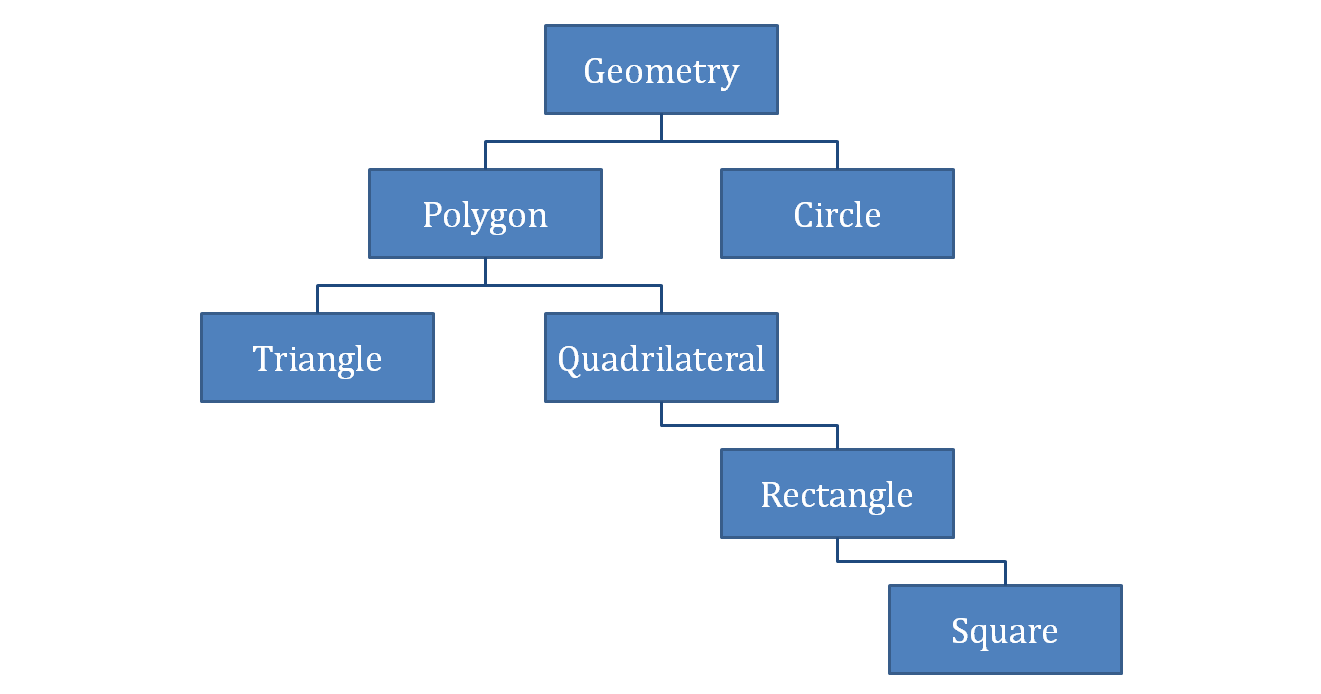
\includegraphics[width=0.8\textwidth]{imgp/classes.png}
\end{center}
\vspace{-2mm}
\caption{Graphical representation of the structure of our classes.}
\label{fig:classes}
\end{figure}

\subsection{Creating sample instances}

Finally let us create sample instances of the classes defined above, inquire
about their areas and perimeters, and let them plot themselves:

\begin{verbatim}
# Create a triangle:
T = triangle([-2, -0.5], [0, -0.5], [-1, 2])
print "Area and perimeter of the triangle:", \
T.area(), T.perimeter()

# Create a quad:
Q = quad([-3, -1], [0, -1], [-1, 1], [-2, 1])
print "Area and perimeter of the quad:", \
Q.area(), Q.perimeter()
 
# Create a rectangle:
R = rectangle(3, 1)
print "Area and perimeter of the rectangle:", \
R.area(), R.perimeter()

# Create a square:
S = square(1.5)
print "Area and perimeter of the square:", \
S.area(), S.perimeter()
 
# Create a circle:
C = circle(2.5, 0, 0.5)
print "Area and perimeter of the circle:", \
C.area(), C.perimeter()

# Plot the geometries:
clf()
T.draw("Triangle")
Q.draw("Quad")
R.draw("Rectangle")
S.draw("Square")
C.draw("Circle")
ylim(-3, 4)
legend()
lab.show()
\end{verbatim}
First, here is the textual output:

\begin{verbatim}
Area and perimeter of the triangle: 2.5 7.38516480713
Area and perimeter of the quad: 4.0 8.472135955
Area and perimeter of the rectangle: 3.0 8.0
Area and perimeter of the square: 2.25 6.0
Area and perimeter of the circle: 19.6349540849 15.7079632679
\end{verbatim}
The graphical output is shown in Fig. \ref{fig:classes2}.

\begin{figure}[!ht]
\begin{center}
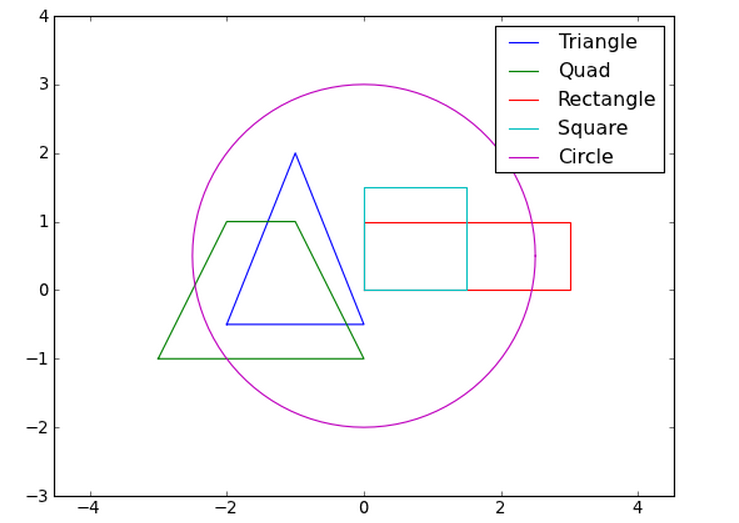
\includegraphics[width=0.82\textwidth]{imgp/classes2.png}
\end{center}
\vspace{-2mm}
\caption{Visualization of the instances created above.}
\label{fig:classes2}
\end{figure}




\subsection{\ \ Programming exercises}

\begin{enumerate}
\item Create a descendant {\tt numberhero} of the class {\tt numbermagic} from Subsection \ref{subsec:obj}
      that in addition to the functionality contained in the class {\tt numbermagic} has one new
      method:
\begin{itemize}
\item {\tt factorize()}: Method that returns a Python list containing primes {\tt p1, p2, ..., pn}
      that form the prime number factorization of the number stored in the object. We recommend 
      that you write a recursive algorithm for the prime number factorization. This is a very 
      nice exercise for recursion.
\end{itemize}
\item Create a descendant {\tt vectorhero} of the class {\tt vectormagic} from Subsection \ref{subsec:obj}
      that in addition to the functionality contained in the class {\tt vectormagic} has one new
      method:
\begin{itemize}
\item {\tt project(V)}: If the two vectors contained in the object form a plane, the 
      method calculates and returns the projection of the vector {\tt V} into this plane. 
      Otherwise the method prints a warning and returns a zero vector. 
\end{itemize}
\item Create a descendant {\tt plottinghero} of the class {\tt plottingmagic} from Subsection \ref{subsec:obj}
      that in addition to the functionality contained in the class {\tt plottingmagic} has two new
      method:
\begin{itemize}
\item {\tt addbezier2(P1, P2, P3, num)}: Method that adds to the database a quadratic B\'ezier curve based 
      on the three control points {\tt P1, P2, P3}. The parameter {\tt num} is a plotting subdivision. 
      See the note below on how B\'ezier curves are defined.
\item {\tt addbezier3(P1, P2, P3, P4, num)}: Method that adds to the database a cubic B\'ezier curve based 
      on the four control points {\tt P1, P2, P3, P4}. 
\end{itemize}
\end{enumerate}
\noindent
{\bf B\'ezier curves}: 

B\'ezier curves are the most widely used approach to define curves in engineering design. 
Let us begin with the linear case. Linear B\'ezier curve is a straight line that
connects two control points $P_1$ and $P_2$. All B\'ezier curves are parameterized
from the interval $[0, 1]$, so in the linear case the exact mathematical definition is
$$
  B(t) = P_1 + t(P_2 - P_1)
$$ 
You can easily check that the curve starts at $P_1$ (substitute $t = 0$ to the above formula),
and that it ends at $P_2$ (substitute there $t = 1$).

Quadratic B\'ezier curves are defined using three control points $P_1, P_2$ and $P_3$. Again they are
parameterized from $[0, 1]$, and their definition is

$$
  B(t) = (1 - t)^2 P_1 + 2(1 - t)t P_2 + t^2 P_3.
$$ 
Cubic B\'ezier curves are defined using four control points $P_1, P_2, P_3$ and $P_4$. They are
parameterized from $[0, 1]$ as usual, and their definition is

$$
  B(t) = (1 - t)^3 P_1 + 3(1 - t)^2t P_2 + 3(1-t)t^2 P_3 + t^3 P_4.
$$ 

\section{Python Libraries}\label{subsec:importinglib}

\subsection{Objectives}

\begin{itemize}
\item Understand that using libraries enhances your problem solving skills.
\item Learn basic facts about Scipy, Numpy, Pylab, Matplotlib, and Sympy.
\item Learn where you can obtain more information about these libraries.
\item Learn that Internet is the best resource for Python programmers.
\end{itemize}
Using libraries is an indivisible part of Python programming. As opposed to 
commercial products, Python libraries are for free. We have used some of them
already, such as Pylab and Matplotlib in Section \ref{sec:calc} and Numpy 
in Section \ref{sec:while}. 

\subsection{Python Standard Library}

The Python Standard Library has vast functionality related to 
built-in functions, built-in types, built-in constants, built-in
exceptions, string services, numerics and mathematics modules, files,
data compression, cryptographic services, and many others. Just introducing 
a table of contents would take several pages. To learn more,
to visit {\tt http://docs.python.org/library/}. Also, a long list of packages for Python 
programmers can be found at {\tt http://pypi.python. org/pypi/}.

\subsection{Pylab and Matplotlib}

The Pylab library can be used for numerical computation but as there are other 
and stronger tools, we recommend to use it mainly for plotting, along with the 
Matplotlib library. For more details on Pylab visit {\tt http://www.scipy.org/PyLab}.
This page is not dedicated to plotting though, more on concrete plotting functionality 
can be found on the home page of Matplotlib, {\tt http://matplotlib.sourceforge.net}.
This page contains an exhaustive overview of plotting-related functionality, many
examples, gallery, and documentation.

\subsection{Scipy and Numpy}

Scipy is a general library for scientific computing with 
Python. Numpy can be viewed as its "heart" containing numerical 
algorithms and methods. These methods comprise interpolation, 
integration, optimization, Fourier transforms, signal processing, 
linear algebra, eigenvalue problems, graph theory routines,
statistics, ordinary and partial differential equations,
image processing, etc. To learn more, visit 
{\tt http://www.scipy.org} and {\tt http://numpy.scipy.org/}. 

\subsection{Sympy}

Sympy is an excellent library for symbolic mathematics covering high-school 
algebra, calculus, matrix algebra and differential equations. To learn more
about Sympy, visit its home page ({\tt http://www.sympy.org}).

\section{Other recommended topics in Python} \label{sec:adv}

There are many topics that we have decided to skip in the first reading 
of the Python language. There is more to learn to almost every command,
function aned concept described in this document. If you like Python,
your nexr resource should be the original Python tutorial at 
{\tt http://docs.python.org}. 




